% This is the main file for the template for doctoral thesis at
% University of Zagreb, Faculty of Electrical Engineering and Computing
% in Zagreb, Croatia.
% Initial version was created in April 2013, last update was in July 2014.

% Author: Jelena Bozek, jelena.bozek@fer.hr
% Contributor: Vedran Miletic, vmiletic@inf.uniri.hr


%%%%%%%%%%%%%%%%%%%%%%%%% POSTAVKE / SETTINGS %%%%%%%%%%%%%%%%%%%%%%%%%%%%%
\documentclass[12pt,oneside, a4paper]{book}
\usepackage{etex}
%\usepackage{xcolor}
\usepackage[pdftex]{graphicx}
\usepackage{rotating}
\usepackage{epsfig}
\usepackage{epstopdf}

% required for printing index
% use \index{name} in text
%\usepackage{makeidx}
%\makeindex
% required for printing nomenclature
% use \nomenclature{symbol}{description} in text
%\usepackage{nomencl}
%\makenomenclature
%\renewcommand{\nomname}{Popis oznaka}

\usepackage[T1]{fontenc}
\usepackage[utf8]{inputenc}
\usepackage{cmap}
\usepackage[english]{babel}
\usepackage{ae}
\usepackage[unicode]{hyperref}
\usepackage{mathptmx}
\usepackage{amscd}
\usepackage{amssymb}
\usepackage{amsmath}
\usepackage{amsfonts}
\usepackage[table]{xcolor}% http://ctan.org/pkg/xcolor
\usepackage{booktabs}

\usepackage[inline]{enumitem}

\setlist[description]{leftmargin=3cm,labelindent=\parindent}
\makeatletter
\def\namedlabel#1#2{\begingroup
    #2%
    \def\@currentlabel{#2}%
    \phantomsection\label{#1}\endgroup
}

\makeatother
% editing a cell 
% https://tex.stackexchange.com/questions/2441/how-to-add-a-forced-line-break-inside-a-table-cell/19678
\usepackage{makecell}
\renewcommand\theadalign{bc}
\usepackage{xspace}


\newcommand{\ComArg}{\mbox{\textsc{ComArg}}\xspace}

\usepackage[left=2.5cm,right=2.5cm,top=2.5cm,bottom=2.5cm]{geometry}
\usepackage{setspace} 
\linespread{1.3}
\usepackage{fancyhdr} % setting up header and position of page numbers
\pagestyle{fancyplain}
\fancyhf{}
\lhead{\nouppercase{\fancyplain{}{\leftmark}}}
\renewcommand{\chaptermark}[1]{\markboth{#1}{}}
\rfoot{\thepage}

\usepackage{minted}
\usepackage{listings}
\usepackage{hhline}
%\usepackage{enumerate}
\usepackage{delarray}
\usepackage{array}  % package for some table properties
\usepackage{tabularx} % package that allows dynamical changing table cell width
\usepackage{multirow}  % package that enables multiple rows in a table
\usepackage[bf, font=small]{caption}
\usepackage[labelfont=small, font=small]{subcaption}
\usepackage{wasysym}
\usepackage{subeqnarray}
\usepackage{aeguill}
\usepackage{pdflscape} % setting page into landscape view
\setlist{nolistsep}   % setting for itemize lists

\usepackage[toc,page]{appendix}

\renewcommand{\thefootnote}{\fnsymbol{footnote}}  % to get unnumbered footnotes
\renewcommand{\arraystretch}{1.5} % stretching row height

\newcounter{rowcntr}[table]
\renewcommand{\therowcntr}{\thetable.\arabic{rowcntr}}

% A new columntype to apply automatic stepping
\newcolumntype{N}{>{\refstepcounter{rowcntr}\therowcntr}c}

% Reset the rowcntr counter at each new tabular
\AtBeginEnvironment{tabular}{\setcounter{rowcntr}{0}}

\usepackage[square, numbers, sort]{natbib} 
% change the name of Bibliography heading into "Literatura"
% \addto\captionscroatian{%
%   \renewcommand{\bibname}{Bibliography}
% }

% Adding a dot after chapter number in TOC 
\let\savenumberline\numberline
\def\numberline#1{\savenumberline{#1.}}

% Adding dots after chapter titles to page number in TOC
\makeatletter
\renewcommand*\l@chapter[2]{%
  \ifnum \c@tocdepth >\m@ne
  \addpenalty{-\@highpenalty}%
  \vskip 1.0em \@plus\p@
  \setlength\@tempdima{1.5em}%
  \begingroup
  \parindent \z@ \rightskip \@pnumwidth
  \parfillskip -\@pnumwidth
  \leavevmode \bfseries
  \advance\leftskip\@tempdima
  \hskip -\leftskip
  #1\nobreak\normalfont\leaders\hbox{$\m@th
    \mkern \@dotsep mu\hbox{.}\mkern \@dotsep
    mu$}\hfill\nobreak\hb@xt@\@pnumwidth{\hss #2}\par
  \penalty\@highpenalty
  \endgroup
  \fi}
\makeatother

% adjust the line spacing in a matrix
\makeatletter
\renewcommand*\env@matrix[1][\arraystretch]{%
  \edef\arraystretch{#1}%
  \hskip -\arraycolsep
  \let\@ifnextchar\new@ifnextchar
  \array{*\c@MaxMatrixCols c}}
\makeatother

% remove footer (page number) from TOC, list of figures and list of tables
\AtBeginDocument{\addtocontents{toc}{\protect\thispagestyle{empty}}}
\AtBeginDocument{\addtocontents{lof}{\protect\thispagestyle{empty}}}
\AtBeginDocument{\addtocontents{lot}{\protect\thispagestyle{empty}}}


\begin{document}


%%%%%%%%%%%%%%%%%%%%%%%%%%%%%%%%%%%%%%%%%%%%%%%%%%%%%%%%%%%%%%%%%%%%%%%%%%%
\frontmatter

%%%%%%%%%%%%%%%%%%%% NASLOVNICA / FRONT COVER PAGE %%%%%%%%%%%%%%%%%%%%%%%%
\begin{titlepage}
  \fontsize{16pt}{20pt}\selectfont
  \fontfamily{phv}\fontseries{mc}\selectfont
  \newgeometry{left=3cm,right=3cm,top=3cm,bottom=2.5cm}
  \setlength{\intextsep}{0pt plus 0pt minus 0pt}

  \begin{center}
    \begin{figure}[ht!]
      \begin{center}
        
\includegraphics[height=4.1184cm, width=5.94cm]{logo_unizg_eng}
      \end{center}
    \end{figure}
    \vspace{0cm}
    {FACULTY OF ELECTRICAL ENGINEERING AND COMPUTING} \\
    \vspace{3cm}
    Filip Boltužić \\
    \vspace{2cm}
    {\fontsize{22pt}{22pt}\selectfont
\textbf{
COMPUTATIONAL METHODS FOR ARGUMENTATION MINING OF CLAIMS IN INTERNET DISCUSSIONS}} \\
    \vspace{2cm}  
    DOCTORAL THESIS \\    
    \vfill{Zagreb, 2019}
  \end{center}
  \restoregeometry
\end{titlepage}

%%%%%%%%%%%%%% DRUGA UNUTARNJA STRANICA / SECOND INNER PAGE %%%%%%%%%%%%%%%
\begin{titlepage}
  \fontsize{16pt}{20pt}\selectfont
  \fontfamily{phv}\fontseries{mc}\selectfont
  \newgeometry{left=3cm,right=3cm,top=3cm,bottom=2.5cm}
  \setlength{\intextsep}{0pt plus 0pt minus 0pt}

  \begin{center}
    \begin{figure}[ht!]
      \begin{center}
        
\includegraphics[height=4.1184cm, width=5.94cm]{logo_unizg_eng}
      \end{center}
    \end{figure}		
    \vspace{0cm}
    {\fontsize{16pt}{16pt}{FACULTY OF ELECTRICAL ENGINEERING AND COMPUTING}} \\
    \vspace{3cm}
    Filip Boltužić \\
    \vspace{2cm}
    {\fontsize{22pt}{22pt}\selectfont\textbf{
COMPUTATIONAL METHODS FOR ARGUMENTATION MINING OF CLAIMS IN INTERNET DISCUSSIONS}} \\
    \vspace{2cm}   
    DOCTORAL THESIS \\  
    \vspace{5cm}   % adjust this spacing if necessary
    Supervisor: Associate Professor Jan Šnajder, PhD \\
    \vfill{Zagreb, 2019}
  \end{center}
  \restoregeometry
\end{titlepage}

%%%%%%%%%%%%%%% PRVA UNUTARNJA STRANICA / FIRST INNER PAGE %%%%%%%%%%%%%%%%
\begin{titlepage}
  \fontsize{16pt}{20pt}\selectfont
  \fontfamily{phv}\fontseries{mc}\selectfont
  \newgeometry{left=3cm,right=3cm,top=3cm,bottom=2.5cm}
  \setlength{\intextsep}{0pt plus 0pt minus 0pt}

  \begin{center}
    \begin{figure}[ht!]
      \begin{center}
        
\includegraphics[height=4.1184cm, width=5.94cm]{logo_unizg2}
      \end{center}
    \end{figure}		
    \vspace{0cm}
    {FAKULTET ELEKTROTEHNIKE I RAČUNARSTVA} \\
    \vspace{3cm}
    Filip Boltužić \\
    \vspace{2cm}
    {\fontsize{22pt}{22pt}\selectfont\textbf{
RAČUNALNI POSTUPCI DUBINSKE ARGUMENTATIVNE ANALIZE TVRDNJI U INTERNETSKIM RASPRAVAMA
}} \\
    \vspace{2cm}    
    DOKTORSKI RAD \\
    \vspace{5cm}    % adjust this spacing if necessary
	Mentor: Izv. Prof. dr. sc. Jan Šnajder \\
    \vfill{Zagreb, 2019.}
  \end{center}
  \restoregeometry
\end{titlepage}


%%%%%%%%%%%%%%%%%%%%%%%%%%%%%%%%%%%%%%%%%%%%%%%%%%%%%%%%%%%%%%%%%%%%%%%%%%%
\begin{titlepage}
  \begin{minipage}{\dimexpr\textwidth-1cm}
    \vspace{3cm}
    Doktorski rad izrađen je na Sveučilištu u Zagrebu
    Fakultetu elektrotehnike i računarstva, na Zavodu za 
    elektroniku, mikroelektroniku, računalne i inteligentne sustave, u 
    Laboratoriju za analizu teksta i inženjerstvo znanja (TakeLab).

    \vspace{1cm}
    Mentor: izv. prof. dr. sc. Jan Šnajder

    \vspace{1cm}
    Doktorski rad ima: XYZ stranica

    \vspace{1cm}
    Doktorski rad br.: \line(1,0){64}
  \end{minipage}
\end{titlepage}

%%%%%%%%%%%%%%%%%%%%%%%%%%%%%%%%%%%%%%%%%%%%%%%%%%%%%%%%%%%%%%%%%%%%%%%%%%%
% insert info page about supervisor which is saved in separate file
\thispagestyle{empty}

\section*{About the Supervisor}


Jan Šnajder has received his BSc, MSc, and PhD degrees in Computer Science from
the University of Zagreb, Faculty of Electrical Engineering and Computing
(FER), Zagreb, Croatia, in 2002, 2006, and 2010, respectively. From September
2002 he was working as a research assistant, from 2011 as Assistant Professor,
and from 2016 as Associate Professor at the Department of Electronics,
Microelectronics, Computer and Intelligent Systems at FER. He was a
visiting researcher at the Institute for Computational Linguistics at the
University of Heidelberg, the Institute for Natural Language Processing at the
University of Stuttgart, the National Instituteof Information and
Communications Technology in Kyoto, and the University of Melbourne. He
participated in a number of research and industry projects in the field of
natural language processing and machine learning. He is the principal
investigator on a HRZZ installation grant project and a HAMAG-BICRO
proof-of-concept project, and a researcher on a UKF project. He has (co-)
authored more than 100 papers in journals and conferences in natural
language processing and information retrieval, and has been reviewing for major
journals and conferences in the field. He is the lecturer in charge for six
courses at FER and has supervised and co-supervised more than 100 BA and MA
theses. He is a member of IEEE, ACM, ACL, the secretary of the Croatian
Language Technologies Society, the co-founder and secretary of the Special
Interest Group for Slavic NLP of the Association for Computational Linguistics
(ACL SIGSLAV). He is a member of the Centre of Research Excellence for Data
Science and Advanced Cooperative Systems and the associate editor of the
Journal of Computing and Information Technology. He has been awarded the Silver
Plaque ``Josip Lončar'' in 2010, the Croatian Science Foundation fellowship in
2012, the fellowship of the Japanese Society for the Promotionof Science in
2014, and the Endeavour Fellowship of the Australian Government in 2015.


\section*{O mentoru}


Jan Šnajder diplomirao je,  magistrirao i doktorirao u polju računarstva na
Sveučilištu u Zagrebu Fakultetu elektrotehnike i računarstva (FER), 2002.,
2006. odnosno 2010. godine. Od 2002. godine radio je kao znanstveni novak, od
2011. godine kao docent, a od 2016. godine kao izvanredni profesor na Zavodu za
elektroniku, mikroelektroniku, računalne i inteligentne sustave FER-a.
Usavršavao se na Institutu za računalnu lingvistiku Sveučilišta u
Heidelbergu, Institutu za obradu prirodnog jezika Sveučilišta u Stuttgartu,
Nacionalnome institutu za informacijske i komunikacijske tehnologije u Kyotu
te Sveučilištu u Melbourneu. Sudjelovao je na nizu znanstvenih i stručnih
projekata iz područja obrade prirodnog jezika i strojnog učenja. Voditelj je
uspostavnog projekta HRZZ-a i projekta provjere koncepta HAMAG-BICRO-a te
je istraživač na projektu UKF-a. Autor je ili suautor više od 100 znanstvenih
radova u časopisima i zbornicima međunarodnih konferencija u području obrade
prirodnog jezika i pretraživanja informacija te je bio recenzentom za veći
broj časopisa i konferencija iz tog područja. Nositelj je šest predmeta na
FER-u te je bio mentorom ili sumentorom studentima na više od 100
preddiplomskih i diplomskih radova. Član je stručnih udruga IEEE, ACM, ACL,
tajnik Hrvatskoga društva za jezične tehnologije te suosnivač i tajnik posebne
interesne skupine za obradu prirodnog jezika za slavenske jezike pri udruzi za
računalnu lingvistiku (ACL SIGSLAV). Član je Znanstvenog centra izvrsnosti za
znanost o podacima i kooperativne sustave te je pridruženi urednik časopisa
Journal of Computing and Information Technology (CIT). Dobitnik je
Srebrne plakete ``Josip Lončar'' 2010. godine, stipendije Hrvatske zaklade za
znanost 2012. godine, stipendije Japanskog društva za promicanje znanosti
2014. godine te stipendije australske vlade Endeavour 2015. godine.


%%%%%%%%%%%%%%%%%%%%%%%%%%%%%%%%%%%%%%%%%%%%%%%%%%%%%%%%%%%%%%%%%%%%%%%%%%%
% insert optional page with thanks or dedication
%\include{eg_thanks_dedication}

%%%%%%%%%%%%%%%%%%%%%%%%%%%%%%%%%%%%%%%%%%%%%%%%%%%%%%%%%%%%%%%%%%%%%%%%%%%
% insert page with abstract
\thispagestyle{empty}

\section*{Summary}

This thesis focuses on several tasks in argumentation mining
of claims. Argumentation mining studies argumentation
extraction from text. With the increase of internet use, 
internet discussions are becoming a valuable source of 
argumentation. Claims constitute the building blocks of
argumentation. 

This research proposes methods for mining topic-specific
argumentative claim analysis in internet discussions. Claims are
structured using a two-level ontology: an upper ontology and a 
domain ontology. The upper ontology is used to describe claim patterns.
The domain ontology models domain-specific concepts. 
Structuring claims allows for higher quality claim
analysis by relaxing the problem of language variance 
and allows for deriving implicit claims. 
Supervised machine learning methods are proposed to detect
and structure claims from internet discussions. 
A method for claim analysis is proposed to analyze
implicit claims of internet discussion participants. 

\vspace{1cm}
\textbf{Keywords}:  
argumentation mining, natural language processing, 
formal knowledge representation, 
structure prediction


%%%%%%%%%%%%%%%%%%%%%%%%%%%%%%%%%%%%%%%%%%%%%%%%%%%%%%%%%%%%%%%%%%%%%%%%%%%
% insert page with extended abstract
% prošireni sažetak na hrvatskom, ako rad nije pisan na tom jeziku
\section*{Sažetak}

\subsection*{Računalni postupci dubinske argumentativne analize tvrdnji u internetskim raspravama}

Rad se bavi nizom zadataka iz područja dubinske analize argumentacije. 
Strukturiranje argumentativnog teksta 
preduvjet je za kvalitetnu analizu argumentacije. 
Potreba za analizom argumentativnog teksta prisutna je u raznim djelatnostima, 
kao što su sažimanje stajališta znanstvenih radova, 
donošenje političkih odluka temeljem javnog mišljenja, 
podučavanje stranog jezika kroz razvoj kritičkog razmišljanja 
i sl. S porastom uporabe interneta sve se više argumentacije nalazi u
internetskim raspravama. Argumentacijom se obrazlaže mišljenje naspram
određene teme. Gradivni elementi argumentacije su argumenti, koji se pak sastoje
od međusobno povezanih tvrdnji. 

Cilj istraživanja bio je razvoj rješenja niza zadataka koji su ključni za 
dubinsku argumentativnu analizu tvrdnji u internetskim raspravama. 
Zadatci uključuju ekstrakciju i strukturiranje tvrdnji tvrdnji. Rješavanje
ovih zadataka vrlo je složeno zbog višeznačnosti jezika i implicitnog 
znanja ovisnog o kontekstu. Pri istraživanju poseban je naglasak bio na izradi
radnog okvira za tematski specifičnu dubinsku argumentativnu rasprave. 
Prvo su provedena tri predistraživanja zasnovana na nestrukturiranim 
metodama dubinske argumentativne analize. Iz predistraživanja detektirani su 
nedostaci nestrukturiranih metoda, stoga je predložen pristup strukturiranja tvrdnji
iskazanih u tekstu, 
koji se smatra najvažnijim doprinosom rada. 

Prvi istražen zadatak u sklopu predistraživanja jest pronalazak istaknutih tvrdnji. 
Potrebno je, uz skup komentara s internetske rasprave, 
pronaći istaknute tvrdnje kojima se sudionici rasprave najčešće služe.  
Prvo se komentari s internetskih rasprava grupiraju u grupe
koje sadrže istovjetne tvrdnje, a centroid grupa pretpostavljen je za 
istaknutu tvrdnju. Komentari se hijarhijski grupiraju koristeći 
njihove distributirane semantičke reprezentacije. 
Rješavanje ovog zadatka olakšava sažimanje rasprave.

Drugi zadatak jest postupak prepoznavanja istaknutih tvrdnji u 
komentarima internetskih rasprava. 
Komentari mogu biti u podupirati ili pobijati istaknute tvrdnje. Prepoznavanje
istaknute tvrdnje svodi se na detekciju odnosa između komentara i tvrdnje. 
Predložen je postupak za prepoznavanje istaknutih tvrdnji 
temeljen na nadziranom strojnom učenju. 

Naposljetku, treći zadatak u sklopu predistraživanja jest 
pronalazak implicitnih informacija u komentarima internetskih rasprava. 
Implicitne informacije između istaknute tvrdnje i komentara koji podupire 
tu istaknutu tvrdnju definirane su putem niza tvrdnji koje upotpunjavaju 
lanac logičkog zaključivanja. Predložene su metode za prepoznavanje istaknutih 
tvrdnji u komentarima uz korištenje implicitnih tvrdnji. 
Pokazano je kako korištenje implicitnih tvrdnji nedvojbeno pospješuje 
rješavanje zadatka prepoznavnaja istaknutih tvrdnji. 
Iz predistraživanja zaključeno je kako je pronalazak implicitnih informacija
bitan za kvalitetnu dubinsku analizu analizu argumentacije. 

Temeljem zaključaka iz predistraživanja, predložen je 
strukturirani pristup pronalaska istaknutih tvrdnji kroz 
radni okvir za strukturiranje tvrdnji. 
U takvome se pristupu definira formalna struktura tvrdnji kako bi se
umanjio problem različitih lingvističkih realizacija u tekstu i omogućilo
izvođenje implicitih tvrdnje logičkim zaključivanjem. 
Strukturirani pristup konceptualno je proveden u tri dijela. 
Prvo je predložena metoda za predviđanje tvrdnji iz komentara, 
zatim su tvrdnje modelirane i strukturirane pomoću računalnih ontologija,
te je, u konačnici, predložen niz metoda zasnovan na strukturiranom 
predviđanju za strukturiranje tvrdnji iz teksta. 

Problem previđanja tvrdnji iz komentara definiran je sukladno srodnim
problemima označavanja sekvenci, kao što je problem ekstrakcije imenovanih
entiteta.  Matematički je definiran problem predviđanja tvrdnji na dva načina.  Za oba načina
predloženo je više modela, među njima i model zasnovan na kombinaciji dubokog
učenja i strukturiranog previđanja. Predloženi modeli eksperimentano su vrednovani 
te je zaključeno kako metode strukturiranog previđanja pomažu
prilikom previđanja tvrdnji. 

S ciljem ublažavanja problema različitih lingvističkih realizacija 
i implicitnosti teksta, 
izdvojene tvrdnje strukturirane su pomoću računalnih ontologija. 
Kroz dvije razine računalnim ontologijama opisuju se tematski specifični koncepti te 
generički obrasci tvrdnji. Kako bi se strukturirale tvrdnje, prvo je 
potrebno definirati tematski specifične koncepte 
za svaku pojedinu temu rasprave, zatim je moguće kombinirati 
definirane koncepte s obrascima kako bi se tvrdnje strukturirale. 

Kako bi se dovršio zadnji korak strukturiranog radnog okvira za dubinsku
argumentativnu analizu predložene su metode za strukturiranje tvrdnji,
zasnovane na nadziranom strojnom učenju. Problem strukturiranja
tvrdnji pokazao se kao vrlo težak problem, uglavnom zbog velikog
broja mogućih rješenja. Eksperimentalnim vrednovanjem najboljim
metodama pokazala se metoda ulančanih klasifikatora,
zasnovanih na strukturiranom previđanju. 

Prednost strukturiranih tvrdnji za dubinsku analizu argumentacije 
demonstrirana je u vidu dohvaćanja implicitnih tvrdnji logičkim
zaključivanjem i grupiranjem sudionika temeljem zajedničkih
tvrdnji u raspravi. Time je pokazan objašnjiv i strukturiran
način pronalaska implicitnih tvrdnji.  

\vspace{1cm}
\textbf{Ključne riječi}:  
dubinska analiza argumentacije, obrada prirodnog jezika,
formalno predstavljanje znanja, 
strojno učenje, strukturirano predviđanje

% prošireni sažetak na engleskom, ako rad nije pisan na tom jeziku
%\include{eg_extended_abstract}

%%%%%%%%%%%%%%%%%%%%%%%%%%%%%%%%%%%%%%%%%%%%%%%%%%%%%%%%%%%%%%%%%%%%%%%%%%%
\clearpage
%%%%%%%%%%%%%%%%%%%%%%%%%%%%%%%%% TOC %%%%%%%%%%%%%%%%%%%%%%%%%%%%%%%%%%%%%
\pagestyle{empty} % remove header/footer 
\tableofcontents
\cleardoublepage % start new page

\pagestyle{fancyplain} % puts headers/footers back on

%%%%%%%%%%%%%%%%%%%%%%%%%%%%%%%%%%%%%%%%%%%%%%%%%%%%%%%%%%%%%%%%%%%%%%%%%%%
\mainmatter
%%%%%%%%%%%%%%%%%%%%%%%% POGLAVLJA / CHAPTERS %%%%%%%%%%%%%%%%%%%%%%%%%%%%%

\chapter{Introduction}

- we argue every day; \\
- Whether it is a domestic discussion which color the bathroom should 
be painted with, a political TV show debate on how will the latest tax increase 
impact small businesses, or a discussion at work on which text editor makes
code editing the fastest, arguments are used to convince the other discussion 
participant(s) to adhere to a single opinion. \\
- More formally, a dialogue or a conversation is defined as a goal-directed
conventional framework in which two partners reason 
together in an orderly way, 
according to the rules of politeness or normal exchange expectations
of cooperative argumentation for the type of exchange they are
engaged in \citep{walton1998new} \\
- from a cooperative and productive argumentative discussion, 
an informed, critically evaluated decision can be made \\
- being able to make important decisions only further 
underlines the importance of argumenation \\
- understanding public opinion on controversial topics, such as 
\textit{marijuana legalization}, \textit{gay marriage legalization}, 
\textit{euthanazia legalization}, and many more is important for
policy making \\
- knowing merely stance (whether someone is pro or con on the topic)
is only surface level information, as arguments behind that stance are
crucial to understance where that stance comes from \\
- analyzing argumentation boils down to understanding and logically connecting
claims into arguments \\
% TODO add claim definition from argonotlogy paper
% - we wish to explore computational methods of 
- we wish to computationally ease the process of analyzing arguments for a 
specific discussion topic \\

%- defining argumentation goes back to Aristotle \\
%- interest in argumentation started with computational argumentation, 
%roughly with \citep{dung1995acceptability} \\

\noindent - computational analysis of arguments started with formalizing arguments, more
specifically, the area of computational argumentation \\
- field of computational argumentation developed formal, logic-based 
accounts of arguments \\
- argumentation is formed in language and therefore related to the field
of computational linguistics \\
- argumentation research has mostly relied on knowledge and 
logic-based solutions, whereas computational lingustics has adopted a 
more , especially with the advent of machine learning \\
- scalability issues limit the application reasoning, logic based
approaches, whereas data-driven approaches often yield non-logical
solutions \\
- one argument towards logic-based approaches 
is that a well-known problem such as POS tagging seems to have reached its
apex with 97\% performance and that rule-based approaches may improve it 
\citep{manning2011part} \\
- we wish to combine logic, reasoning-basec approaches with data-driven ones \\

\noindent - our goal is to allow for argument analysis from raw text \\
- the text is expected to be from online discussions, more specifically internet 
discussions, which carry have their own set of rules and conventions \\
- we wish to work on problems to extract claims, group claims into arguments, and analyze 
claims, potentially deriving new claims (premises) \\

% - in this work we wish to balance between formalized and unformalized approaches \\
% - we aim to use non-formalized approaches to identify and extract claims from text, then use
% formalized and structured approaches to derive arguments from claims along with their
% underlying premises of arguments \\

\section{Argumentation Mining of Claims}

- argument analysis is performed from many angles \\
- computational argumentation starts with predefined claims and connects them 
with (support or attack) relations to form arguments and networks of arguments \\
- these argument networks (graphs) are then usually analyzed in terms of acceptability \\
- however, this approach can be rather expensive, as no automatic methods currently exist
to determine claims \\
- argumentation mining relies on natural language processing techniques to
extract claims from text, recognize relations between claims and then analyze them
by means of clustering on deriving extra claims (or premises) from 
extracted ones \\
- we wish to walk the line between argumentation mining and computational argumentation 
by extracting claims by means of natural language processing, after which we 
experiment with both structured and unstructured approaches of claim analysis \\

\section{Contributions}

% TODO this is from the javni razgovor document
The research aims to improve the state of
the art in argumentation mining by means of claim structuring and the
development of a computer system prototype for claim analysis, which would
allow for better understanding of argumentation in internet discussions. 
The prospective original scientific contribution consists of: 
\begin{enumerate}
\item A method for modeling of argumentation in internet discussions using an
two-level ontology, where the first level contains topic-specific knowledge,
while the second level models the claim patterns;
\item A computational method for detection and
structuring of claim in argumentative discourse based on supervised machine
learning;
\item A framework and a prototype of a system for computer-aided
analysis of claims in internet discussions which links together the detection,
structuring, and the analysis of claims.  
\end{enumerate}

\section{Thesis structure}

The thesis is structured as follows. Finally, chapter~\numberstringnum{\getrefnumber{chap:conclusion}}
concludes the thesis and gives directions for future work. 

% 


\chapter{Uvod}

U ovom poglavlju prikazane su neke od funkcije koje se mogu koristiti prilikom
oblikovanja rada i prikaza rezultata istraživanja korištenjem \LaTeX a.

\section{Matematički izraz}


Primjer matematičke formule prikazan je izrazom

\begin{equation}
  T: \mathbf{x}_B \mapsto \mathbf{x}_A \Leftrightarrow T(\mathbf{x}_B) = \mathbf{x}_A.
  \label{eq:transformacija}
\end{equation}


\section{Slika}


Slika \ref{fig:roc_example} služi kao primjer ubacivanja slike u tekst.

\begin{figure}
  \centering
  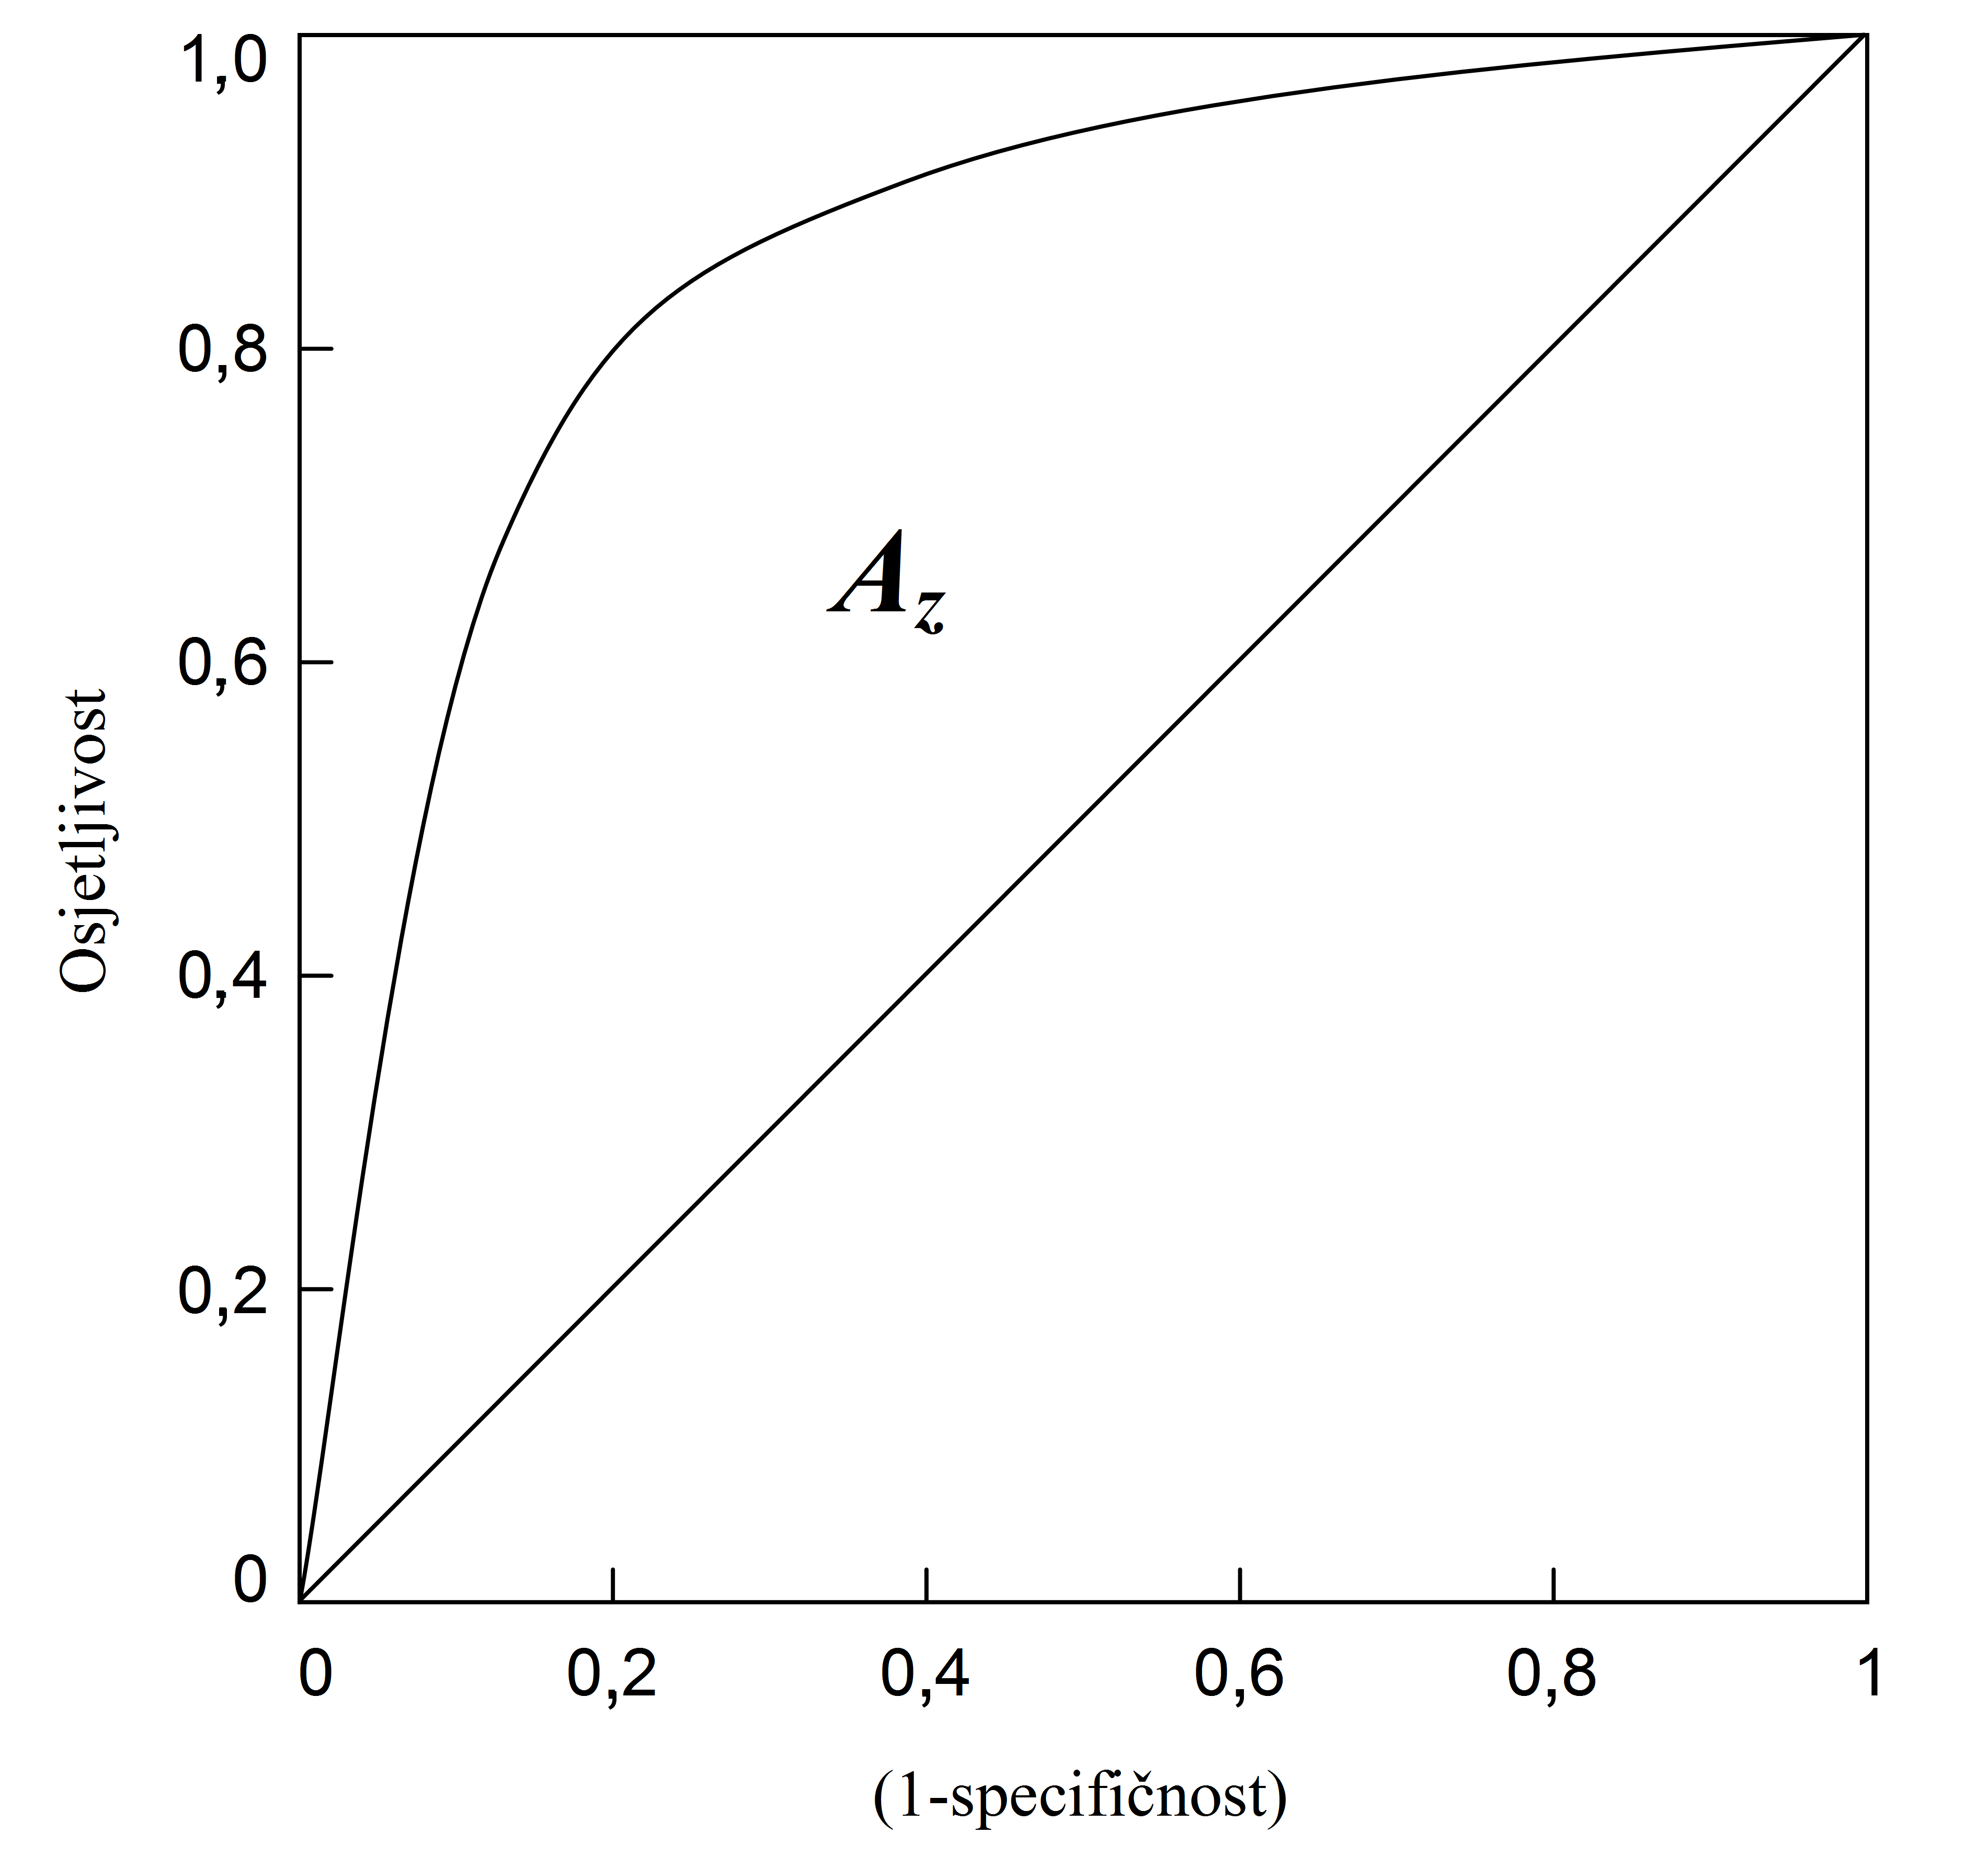
\includegraphics[width=0.7\textwidth]{roc_example}
  \caption{Primjer krivulje ROC}
  \label{fig:roc_example}
\end{figure}


\section{Tablica}


Formiranje tablice prikazano je na primjeru matrice podudarnosti u Tablici
\ref{tab:confusion_matrix}.

\begin{table} [!ht]
  \caption{Matrica podudarnosti}
  \centering  
  \begin{tabularx}{0.5\textwidth}{ c  c | c | c |}

    \cline{3-4}
    & & \multicolumn{2}{c|} {Predviđeno (\textit{predicited})}  \\ \cline{3-4}
    & & Negativno & Pozitivno \\ \cline{1-4}
    \multicolumn{1}{ |c } {\multirow{2}{*}{\rotatebox{90}{\parbox[c]{1.4cm} {Stvarno \\ (\textit{actual})}}}}  & \multicolumn{1}{ |c| }{Negativno} & NN & LPN \\ \cline{2-4}
    \multicolumn{1}{ |c  }{} & \multicolumn{1}{ |c| }{Pozitivno} & LNN & PN \\ \cline{1-4}

  \end{tabularx}
  \label{tab:confusion_matrix}
\end{table}

\subsection{\textit{Landscape}}

Postavljanja stranice u prikaz \textit{landscape} prikazano je umetanjem Tablice \ref{tab:mean_mias} u \textit{landscape}. Prikazano je i dodavanje \textit{footnotea} u tablicu.

\begin{landscape}
  \begin{table}
    % tekst u uglatim zagradama koje slijede \caption prikazuje se u Popisu tablica, a tekst u vitičastim zagradama koje slijede \caption prikazuje se iznad same tablice
    \caption[Srednje vrijednosti mjera sličnosti slika za bazu
	  mini-MIAS]{Srednje vrijednosti mjera sličnosti lijevog i desnog
	  mamograma prije i poslije registracije vođene različitim funkcijama
	  troška. Rezultati su prikazani za asimetrične (A) i normalne (N)
	  slučajeve u bazi mini-MIAS.}
    \begin{minipage}{\linewidth}   %minipage adjusts for its own footnotes
      \setcounter{mpfootnote}{\value{footnote}}
      \renewcommand{\thempfootnote}{\fnsymbol{mpfootnote}} 
      % \makebox[\textwidth] {          % center table on the page since it's wider than the page margins
      \newcolumntype{C}{>{\centering\arraybackslash}X}%
      \begin{tabularx} {\linewidth}{l C C C C C C C C C C C C} %{ c c c c c c c c c c c c c} 
        \multirow{2}{*}{\textbf{Mini-MIAS}} & \multicolumn{2}{c}{\textbf{SSD}} & \multicolumn{2}{c}{\textbf{CC}} & \multicolumn{2}{c}{\textbf{MI}} & \multicolumn{2}{c}{\textbf{NMI}} & \multicolumn{2}{c}{\textbf{SSIM}} & \multicolumn{2}{c}{\textbf{KLD}} \\  \cline{2-13}
        & \multicolumn{1}{c}{\textbf{A}} & \multicolumn{1}{c}{\textbf{N}} & \multicolumn{1}{c}{\textbf{A}} & \multicolumn{1}{c}{\textbf{N}} & \multicolumn{1}{c}{\textbf{A}} & \multicolumn{1}{c}{\textbf{N}} & \multicolumn{1}{c}{\textbf{A}} & \multicolumn{1}{c}{\textbf{N}} & \multicolumn{1}{c}{\textbf{A}} & \textbf{N} & \multicolumn{1}{c}{\textbf{A}} & \multicolumn{1}{c}{\textbf{N}} \\ \cline{1-13} %\hline

        Prije reg.  & 797,01 & 765,67  & 0,93 & 0,92 & 0,86 & 0,80 & 1,19 & 1,21 & 0,84 & 0,87 & 0,21 & 0,14 \\ \cline{1-13}
        Reg. sa SSD & 706,37 & 556,18  & 0,94 & 0,94 & 0,91 & 0,88 & 1,20 \footnotemark[1] & 1,24 \footnotemark[1] \footnotemark[2] & 0,86 \footnotemark[1] & 0,89 \footnotemark[1] & 0,20 & 0,14 \\ \cline{1-13}
        Reg. s CC   & 691,18 & 520,68  & 0,94 & 0,95 & 0,91 & 0,87 & 1,20 \footnotemark[1] & 1,23 \footnotemark[1] & 0,86 \footnotemark[1] & 0,89 \footnotemark[1] & 0,20 & 0,14 \\ \cline{1-13}
        Reg. s MI   & 840,84 & 649,41  & 0,92 & 0,93 & 0,92 & 0,87 & 1,21 \footnotemark[1] & 1,23 \footnotemark[1] & 0,86 \footnotemark[1] & 0,88 \footnotemark[1] & 0,20 & 0,14  \\ \cline{1-13}
        Reg. s NMI  & 758,53 & 572,00  & 0,93 & 0,94 & 0,92 & 0,86 & 1,21 & 1,23 & 0,86 \footnotemark[1] & 0,88 \footnotemark[1] & 0,20\footnotemark[2] & 0,14 \\ \cline{1-13}

      \end{tabularx} 
      \footnotetext[1]{statistički značajna razlika između asimetričnih i normalnih slučajeva za istu mjeru sličnosti}
      \footnotetext[2]{statistički značajna razlika u odnosu na vrijednost prije registracije za istu mjeru sličnosti} 
      % }
      \label{tab:mean_mias}
      \setcounter{footnote}{\value{mpfootnote}}
    \end{minipage}
  \end{table}
\end{landscape}


\section{Primjeri literature}


Popis literature navodi se na kraju doktorskog rada. Primjeri navođenja
literature su knjiga \cite{Hajn01}, poglavlje u knjizi \cite{Samp05}, članak
objavljen u časopisu \cite{Sim03}, članak objavljen na konferenciji
\cite{Wirt99}, doktorski rad \cite{Will93}, Internetski izvor \cite{Jone12} te
različite druge publikacije \cite{Rsoft}. Stil navođenja literature temelji se
na stilu razvijenom za IEEE časopise i konferencije, autora Michaela Shella uz
unesene prilagodbe stila za doktorski rad pisan na FER-u.



%%%%%%%%%%%%%%%%%%%%%%%% PRILOZI / APPENDIX %%%%%%%%%%%%%%%%%%%%%%%%%%%%%%%

%\appendix
%\addcontentsline{toc}{section}{Appendices}
%\renewcommand{\thechapter}{A}
%\renewcommand{\thesection}{\Alph{section}}
%\setcounter{section}{0}

\begin{appendices}

\chapter{Text Datasets}
\label{chap:appendix_datasets}

Here is the list of all the datasets created as part of this thesis.

\begin{enumerate}[label=\textbf{A.\arabic*}]
\item\label{item:comarg} \ComArg is a dataset of online user comments manually annotated with
comment-argument pairs. The dataset is created for the argument
recognition task: identifying what arguments, from a predefined
set of arguments, have been used in users' comments, and how.
It consists of 1285 and 1013 comment-argument pairs from 
on-line discussions of \emph{Gay Marriages} (GM) 
and \emph{Under God in pledge} (UGIP) respectively.
The dataset is publicly available at:
\url{http://takelab.fer.hr/data/comarg/}

\item\label{item:argpremises} ArgPremises is a dataset of 
implicit premises manually annotated on matching claims. 
The dataset is created to explore what are the implied premises users 
make when expressing support for a claim.
Additionally, it was used to help solve the claim matching task; 
using implicit premise information whilst 
identifying whether a pair of claims expresses the same argument. 
It consists of 494 claim pairs and 3977 respective premises on topics
of \emph{Marijuana Legalization} (MA), \emph{Gay Rights} (GA), 
\emph{Abortion Legalization} (AB),
and \emph{Obama Presidency} (OB).
The dataset is publicly available at:
\url{http://takelab.fer.hr/data/argpremises/}

\item\label{item:microstructures_dataset} 
The Claim Microstructure dataset contains online
discussion comments split into claim
segments, translated into claim microstructures. The dataset is created
to explore how claims can be structured using a restricted
language and grammar. Additionally, it was used to help solve
the stance classification task; using claim microstructure
information when determining stance of a claim. 
The dataset consists of 
100 user posts on the ``\emph{Gay Rights}'' (GA) topic, 
split into 920 claim segments and paraphrases, which two people
(A1 and A2) annotated
882 microstructures (A1) and 842 microstructures (A2), and a hierarchical 
list of 307 concepts used to form microstructures. 
The dataset is publicly available at:
\url{http://takelab.fer.hr/claim-micro}

\item\label{item:structure_dataset} 
Similarly to the microstructure dataset, 
the ontology formalization dataset also contains online discussion
comments split into claims and translated to claim formalizations.
The claim formalizations are logical representations of claims
and may be used to logically derive implicit claims.
The formalization is defined by a two-level ontology: an upper and 
a domain ontology. 
The dataset consists of 100 user comments on the ``\emph{Marijuana}''
split into 920 claim segments and paraphrases. 
The domain ontology for the topic consists of 75 domain
individuals. Three people annotated the claim segments with 
864 (A1), 867 (A2), and 860 (A3) claim individual formalizations.

\end{enumerate}


\chapter{Annotation Guidelines}
\label{chap:annotation_guidelines}

Quality labelled annotated datasets are essential to build and evaluate argumentation
mining models.  High quality dataset annotation requires that annotators are
well trained in the task at hand. 
Data should be consistently annotated between indepedently working annotators. 
To ensure annotators understand the assigment and are able to complete 
the annotation task successfully, good annotation guidelines are required. 
During the annotation of data described in this thesis  
annotators had to do a test annotation before the real one, 
discuss differences until resolution, and redo annotation of examples
where there was no consensus. 
Once the annotation is complete, we measure inter-annotator agreement. 
In the case of two annotators that each classify $N$ items into $k$ mutually
exclusive categories, we use the Cohen's kappa \citep{cohen1960coefficient}. 
Cohen's kappa is defined as
$$
\kappa = \frac{p_0 - p_e}{1 - p_e}
$$
where $p_0$ is the relative observed agreement among annotators, and 
$p_e$ is the hypothetical probability of chance agreement. 
We use Fleiss' kappa to asses inter-annotator agreement when dealing with more than
two annotators \citep{fleiss1993review}.
Let $N$ be the number of annotators, $n$ number of ratings per subject, and
$k$ number of categories into which assignments are made. Then $n_{ij}$ represents
the number of annotators who assigned $i$-th subject to the $j$-th category. 
Fleiss' kappa is defined the same as Cohen's kappa, but $p_0$ and $p_e$ are defined as:
\begin{align*}
p_0 &= \frac{1}{Nn(n-1)} \left( \sum_{i=1}^{N} \sum_{j=1}^{k} n_{ij}^2 - Nn \right) \\
p_e &= \frac{1}{Nn} \sum_{j=1}^{k} \left( \sum_{i=1}^{N} n_{ij} \right)^2
\end{align*}

This chapter shows the annotation guidelines for 
\begin{enumerate*}[label=(\arabic*)]
\item microstructures (Section~\ref{sec:microstructure_annotation_appendix}), 
\item argumentative segments (Section~\ref{sec:argseg_annotation}),
\item prominent claim and claim relationship pairs (Section~\ref{sec:argrec_annotation}),
\item claim set similarities, (Section~\ref{app:sec:argpremises_annotation}), and
\item claim formalizations (Section~\ref{sec:formalization_annotation}).
\end{enumerate*}

\section{Microstructure annotation guidelines}
\label{sec:microstructure_annotation_appendix}

\noindent - Microstructures represent logically structured argumentative claims
\citep{boltuzic2017toward}. \\
- One can expresses logically equivalent claims in language \\
- To limit the language variation microstructures were designed to translate
expression rich phrases to be translated to a restricted language to allow for
easier inference \\
- microstructures  consist of domain specific concepts, 
connected through a finite set of argumentative relations, expressed using 
a certain modality \\
- microstructure annotation proceduced the microstructures data (
see item element in \ref{item:microstructures_dataset})\\

\newpage
\subsection{Cheat sheet}

\begin{minted}{microstructure_lexer.py:MicroStructureLexer -x}
viewpoint_1(
	viewpoint_2[holder](
		relation_1([quantity_1] concept_1, [quantity_2] concept_2)
	)
)

concept_1 = concept OR relation_2(concept_3, concept_4)
concept_2 = concept OR relation_3(concept_5, concept_6)

\end{minted}

\noindent \textbf{Viewpoints} \\
- Believes, Approves, Disapproves, Desires

\begin{minted}{microstructure_lexer.py:MicroStructureLexer -x}
viewpoint_1(
	relation_1(relation_2(concept_3, concept_4), concept_2)
)
\end{minted}

\noindent \textbf{Relations} (grayed columns indicate dual meaning between relations in each row)

\begin{table}[!htb]
\begin{tabular}{|c c c c c c|}
\hline
\cellcolor{gray!25} \texttt{promotes} & \cellcolor{gray!25}\texttt{allow} & \texttt{purpose} & \texttt{equal} & \cellcolor{gray!25}\texttt{entails}     & \texttt{has\_associated} \\
\cellcolor{gray!25} \texttt{suppress} & \cellcolor{gray!25}\texttt{deny}  &         &       & \cellcolor{gray!25}\texttt{contradicts} &  \\
\hline
\end{tabular}
\end{table}

\noindent \textbf{Negation} (use with relations)
Use with relation in front (\texttt{not\_promotes}, \texttt{not\_suppress}, \dots) \\
 
\noindent \textbf{Quantities} (use with concepts) \\
Some, All, Minority, Majority \\
          
\noindent \textbf{Concepts} 
\footnote{\url{https://docs.google.com/document/d/1ETobyCA4mpMmml1HXyxD7IG67EzrNK7W_2gzaIN0k_k/edit}} \\

\noindent \textbf{Quality} $\in [1, 5]$ \\
 
\noindent \textbf{Stance} $ \in {-2, -1, 0, 1, 2}$ \\

\pagebreak

\subsection{Task description}

In this task we annotate argumentative sentences/claims and represent them
using a logical generative grammar language, as well as a stance. The
argumentative sentences are paraphrases of debate post excerpts. We will
provide you with the original post, as the argumentative sentences provided
might not be enough to fully understand the meaning. 
The language has a set of syntactic rules, which need to be respected. The
syntax of your solutions will be checked as you annotate the document. 
An example sentence will look like:
\noindent\begin{tabular}{@{}lp{0.8\columnwidth}}
(ex. 1) & \textit{Homosexual marriage can not truly be a marriage.}
\end{tabular} \vspace{0.4cm}

\noindent We want to translate this to the form of: 

\begin{tabular}{@{}m{1.5cm}  m{4.5cm}}
(ex. 1) &  \begin{minted}{microstructure_lexer.py:MicroStructureLexer -x}
believes(
    contradicts(homosexual marriage, marriage)
)
\end{minted}
\end{tabular}

In this context, we call homosexual marriage and marriage concepts. The element
contradicts is a relation between the concepts. Believes is a viewpoint that
depicts the author's perspective. See more on concepts, relations and
viewpoints in the language description section below. 

Good practice when creating these annotations is attempting to read them back
in natural language. In this case, we get: I believe that homosexual marriage
is not marriage.  If we compare this to the original sentence, we see that it
captures the essence of the example sentence (ex. 1). The wording is lost,
which can mean a lot sometimes (reading between the lines), but this is
something we’re OK with.

\subsection{Language description}

As said, we annotate:
\begin{itemize}
\item Concepts
\item Relations between concepts
\item Viewpoints
\end{itemize}

\subsubsection{Concepts}

Concepts are noun phrases mentioned when discussing a topic. We provide a set
of concepts that we have previously identified for the ``gay rights'' topic\footnote{
Concepts available at 
\url{https://docs.google.com/document/d/1ETobyCA4mpMmml1HXyxD7IG67EzrNK7W_2gzaIN0k_k/edit?usp=sharing}
}
Some concepts are tab-shifted, which you can disregard, some have
slashes between them (i.e. \texttt{heterosexual marriage} / \texttt{traditional marriage}); we
consider these synonyms, please choose the first one. Your task is to search
through this list and find appropriate concepts (as close concept as possible)
mentioned in the input sentence and associate the appropriate relations between
them. Some example concepts: \texttt{procreation}, \texttt{reproduction}, \texttt{adoption}, \texttt{homosexual}
\texttt{adoption}, \texttt{have children}, \texttt{gay people}. 
If you feel you need to use a concept not
in the list, please contact us with the example. Another case would be where a
concept might be implicit, in the sentence: \textit{Allow gay marriages}, we recognize
the relation \texttt{allow} (explained in relations below) and the concept \texttt{gay marriages}
(argument B for relation \texttt{allow}).  We don’t know what the principle is, but from
the topic we know the state can allow gay marriages, therefore we can translate
the sentence as: \texttt{allow(state, gay marriage).}

\subsubsection{Quantity}

Each concept can be expressed with quantity. Quantities allowed are:
\begin{itemize}
\item Some 
\item All
\item Minority
\item Majority
\end{itemize}

\begin{table}[!htb]
\begin{tabular}{@{}m{1.5cm} m{5cm} m{8cm}}
\toprule
Example & Sentence & Microstructure \\
\midrule
(ex. 2.a) & Some people promote gay marriages. & 
\begin{minted}{microstructure_lexer.py:MicroStructureLexer -x}
believes(
  promote([some]people, gay marriage)
) 
\end{minted}
\\
(ex. 2.b) &Democracy helps the majority of people. &
\begin{minted}{microstructure_lexer.py:MicroStructureLexer -x}
believes( 
  promote(democracy, [majority] people)
)
\end{minted} 
\\
\bottomrule
\end{tabular}
\end{table}

\subsubsection{Relations}

Relations are connections between concepts. Relations are not domain-bound (one
can use them outside of gay marriages), while concepts are tied to domain 
(\texttt{gay marriages} in this case). Relations are verb phrases. 
Possible relations are:

\begin{footnotesize}
\begin{tabular}{lp{5cm}p{2.5cm}p{3cm}}
\toprule
Relation & Explanation & Argument A & Argument B \\
\midrule
\texttt{promotes(A, B)} & 
\makecell[cl]{
\textbf{A} promotes / fosters / \\
brings about / leads \\ 
/ forces / advances \\
/ increases /encourages \\
/ boosts / increases \\
the likelihood of / causes \textbf{B}  \\ \\
``Soft causation'' \\\\
\href{https://framenet2.icsi.berkeley.edu/fnReports/data/frameIndex.xml?frame=Cause_change_of_position_on_a_scale}{FrameNet link} 
}
& 
Agent (which promotes) & 
Attribute (what gets promoted) \\
\midrule
\texttt{suppress(A, B)} & 
\makecell[cl]{
\textbf{A} suppresses / decreases \\ 
likelihood / smothers / \\
represses / puts down / \\
vaniquishes \textbf{B} 
}
&
Agent (which suppresses) & 
Attribute (what gets suppressed)
\\
\midrule
\texttt{allow(A, B)} & 
\makecell[cl]{
Principle \textbf{A} \\ 
allows / approves / \\
licenses \textbf{B} \\\\
\href{https://framenet2.icsi.berkeley.edu/fnReports/data/frameIndex.xml?frame=Prohibiting_or_licensing}{FrameNet link}
} & 
Principle
& 
State of affairs \\
\midrule
\texttt{deny(A, B)} & 
\makecell[cl]{
Priciple \textbf{A} \\
denies / disallows /
bans \textbf{B} } & 
Principle & 
State of affairs\\
\midrule
\texttt{entails(A, B)} & 
\makecell[cl]{
State of affairs \textbf{A} \\
necessarily, per definition \\
or causally, makes \textbf{B} true \\\\
Proposition \textbf{B} has \\
support \textbf{A} \\\\
\href{https://framenet2.icsi.berkeley.edu/fnReports/data/frameIndex.xml?frame=Evidence}
{FrameNet link}
}
& State of affairs & Implication \\
\midrule
\texttt{contradicts(A, B)} & 
\makecell[cl]{
State of affairs \textbf{A} \\
makes \textbf{B} not true}
& State of affairs & Contradiction \\
\midrule
\texttt{purpose(A, B)} & 
\makecell[cl]{The purpose of \textbf{A} is \textbf{B} \\\\
\href{https://framenet2.icsi.berkeley.edu/fnReports/data/frameIndex.xml?frame=Purpose
}{FrameNet link}
} & Agent & Goal \\
\midrule
\texttt{has\_associated(A, B)} &
\makecell[cl]{
\textbf{A} has properties affected by \\
the existence of \textbf{B} \\\\
\href{https://framenet2.icsi.berkeley.edu/fnReports/data/frameIndex.xml?frame=Membership
}
{Similar FrameNet definition} 
} & Group & Member \\
\midrule
\texttt{equal(A, B)} & \textbf{A} is equal to \textbf{B} & Concept \textbf{A} & Concept \textbf{B} \\
\bottomrule
\end{tabular}
% \caption{Relation definition table}
% \label{tab:relation_definition}
% \end{table}
\end{footnotesize}

\subsubsection{Negation}
%TODO proper references in table rows

Relations can be negated to indicate opposite meaning. Notice how example $3.a$
is not saying it is suppressing, but just denied promoting. Example $3.b$ also can’t
use contradicts since being happy does not imply you are not rich, but it does
not imply you are.

\begin{footnotesize}
\begin{tabular}{@{}m{1.5cm} m{5cm} m{8cm}}
\toprule
Example & Sentence & Microstructure \\
\midrule
(ex. $3.a$) & \textit{Marijuana does not help cure cancer. } & 
\begin{minted}{microstructure_lexer.py:MicroStructureLexer -x}
believes(
  not_promotes(marijuana, cure cancer)
)
\end{minted}
\\
(ex. 3.b) & \textit{If you are happy, doesn’t mean you’re rich.} 
 &
\begin{minted}{microstructure_lexer.py:MicroStructureLexer -x}
believes(
  not_entails(feel happy, be rich)
)
\end{minted} 
\\
\bottomrule
\end{tabular}
\end{footnotesize}

\subsubsection{Nested Relations}

Relations can be nested within each other. Each relation takes two arguments.
An argument can be another relation or a concept. Make sure you are correct
with closing the opened braces. 

\begin{footnotesize}
\begin{tabular}{@{}m{1.5cm} m{5cm} m{8cm}}
\toprule
Example & Sentence & Microstructure \\
\midrule
(ex. $4.a$) & \textit{I think allowing gay marriages promotes freedom. } & 
\begin{minted}{microstructure_lexer.py:MicroStructureLexer -x}
believes(promotes(
  allow(state, gay marriage), freedom
  )
)
\end{minted}
\\
(ex. 4.b) & \textit{The purpose of life is to allow having freedom.} 
 &
\begin{minted}{microstructure_lexer.py:MicroStructureLexer -x}
believes(
  purpose(life, 
    allow(state, freedom)
  )
)
\end{minted} 
\\
(ex. 4.c) & \textit{It’s the same thing to allow gay marriages or heterosexual marriages.} & 
\begin{minted}{microstructure_lexer.py:MicroStructureLexer -x}
believes(
  equal(
    allow(state, gay marriage), 
    allow(state, heterosexual marriage)
  )
)
\end{minted}
\\
\bottomrule
\end{tabular}
\end{footnotesize}

\subsubsection{Viewpoints}

Viewpoints reflect whether the a viewpoint holder thinks the claim is believed
(fact), desired (policy), or considered right/wrong (value judgement). When not
mentioned, the claim holder is considered to be the author of the argumentative
sentence. If not, one needs to annotate the claim holder next to the viewpoint
type (\textit{I believe the Bible states}, \textit{I think the state of Florida should}), which
we call second-level viewpoints. Second-level viewpoints are annotated together
with a concept, for example: "\textit{I saw that the Bible states: It should be
allowed}" corresponds to "\texttt{believes(believes[Bible]...))}".
Possible viewpoints are \\

\begin{tabular}{l p{7cm} p{6cm}}
\toprule
Viewpoint & Description & Example \\
\midrule
\textbf{believes} & \textbf{A} believes / argues / thinks
that claim \textbf{C} is true & 
I believe people are mortal. \\
\midrule
\textbf{desires} & 
\textbf{A} believes / argues / thinks \textbf{C} 
should be true in the future or should remain true
& People should be nicer \\
\midrule
\textbf{approves} & 
\textbf{A} believes / argues / thinks \textbf{C} 
is morally / ethically right & Forgiving is bad \\
\midrule
\textbf{disapproves} & 
\textbf{A} believes / argues / thinks \textbf{C} 
is morally / ethically wrong & 
Drugs are bad.  \\
\bottomrule
\end{tabular} \\
% \label{tab:viewpoints}
% \caption{Viewpoints, their descriptions and examples of using specific viewpoints in claims}

\noindent Annotating a claim holder explicitly should be done like for sentence:

\begin{table}[h]
\begin{tabular}{@{}m{1.5cm} m{5cm} m{8cm}}
\toprule
Example & Sentence & Microstructure \\
\midrule
(ex. $5.a$) & \textit{I saw the Bible claims gay people are equal to straight people} & 
\begin{minted}{microstructure_lexer.py:MicroStructureLexer -x}
believes(
  believes[Bible](
    equal(gay people, straight people)
  )
)
\end{minted}
\\
\bottomrule
\end{tabular}
\label{tab:viewpoint_example}
\caption{Viewpoint claim annotation example}
\end{table}

\subsubsection{Stance}

Please annotate stance, which answers the question:
\textbf{Is the sentence pro-gay or not just by looking only at the offered claim} (not
the entire post context)? Stance $\in {-2, -1, 0, 1, 2}$.

\begin{table}[!htb]
\begin{tabular}{c p{10cm}}
\toprule
Stance Value & Explanation \\
\midrule
-2 & The author or the viewpoint of the second person is definitely against the
claim (explicitly states so). Any form of discrimination is seen as against.  \\
-1 & There is some implication that the author might be against gay rights  \\
0 & There is no stance towards gays, stance is bipolar \\
1 & Reverse of -1 \\
2 & Reverse of -2 \\
\bottomrule
\end{tabular}
\label{tab:stance}
\caption{Possible stance values with explanations}
\end{table}

\begin{table}[!htb]
\begin{tabular}{c p{10cm} r}
\toprule
Example & Claim & Stance \\
\midrule
(ex. $6.a$) &  I think allowing gay marriages promotes freedom. & 2 \\
(ex. $6.b$) & All people are equal. & 0 \\
(ex. $6.c$) & Allowing gay marriages will be the end of us all. &  -2 \\
(ex. $6.d$) & I would ban religious gay marriage. & -2 \\
(ex. $6.e$) & The Bible is against gay marriages & -2 \\
\bottomrule
\end{tabular}
\label{tab:stance_example}
\caption{Examples of stance for the gay marriages topic}
\end{table}

\subsubsection{Quality}

Evaluate your own logical claim transformation by inputting a number $\in [1, 5]$
rating how well does the proposed formalization suit what the person said?

\subsection{Technical instructions}

You will be provided with an excel spreadsheet with the posts and sentences.
Please notify us as soon as possible if you can’t use Excel - we can send you
the annotation in another format (Google spreadsheet, etc.). 

The goal is to fill up the E, F, G columns (logical representation, stance and
quality, highlighted in green) in the provided spreadsheet based on the
argumentative sentence in column D. Feel free to ignore columns A, and C (used
for internal tracking). Column B might be useful, if you can’t determine the
meaning in D. If you have problems or comments about an example, feel free to
add them in column H and raise questions with us -- we will be happy to
discuss! An example row will look like in table~\ref{tab:annotation_example}

\begin{table}[!htb]
\scriptsize
\begin{tabular}{|p{1.5cm} | p{2cm} | p{2cm} | p{2cm} | p{2cm} |c| c| c|}
\toprule
A & B & C & D & E & F & G & H \\
\midrule
POST ID & POST TEXT & SEGMENT ID & SENTENCE & LOGICAL REPRESENTATION
& STANCE & QUALITY & COMMENTS \\
\midrule
A75.data & 
Here we is the full text of the post. This will be relatively long.
This is divided into segments (argumentative sentences) that you then annotate. 
& 758 & 
The full text of the post will be relatively long.  
& \cellcolor{green!25} &  \cellcolor{green!25}& \cellcolor{green!25} & \cellcolor{green!25} \\
\bottomrule
\end{tabular}
\caption{Example excel sheet to annotate}
\label{tab:annotation_example}
\end{table}

A syntax checking script and your annotation is packaged into a zip file.  Your goal is to
fill column E in \texttt{annotation.xls}.

\subsubsection{Checking syntax correctness (optional)}

We provide a script to verify that your solutions are syntactically correct. 
You will need to install python and a python library xlrd. Make sure to install
\texttt{python 2.x}!

If you are not familiar with python, installing them on Windows is desribed in
\url{http://www.howtogeek.com/197947/how-to-install-python-on-windows/}
Xlrd is available to install from:
\url{http://www.lexicon.net/sjmachin/xlrd-0.6.1.win32.exe} 
To install it, you will need to Run-as-administrator. 
Please contact us if you have issues installing these. 
To help check correctness of your solution, we offer a python script that can
be run in two ways:

\begin{description}[style=multiline, labelwidth=1.5cm]
\item[\namedlabel{item:excel}{All}] Check all solutions in your excel spreadsheet
\item[\namedlabel{item:single_claim}{Single}] Check a single claim
\end{description}

\begin{figure}
	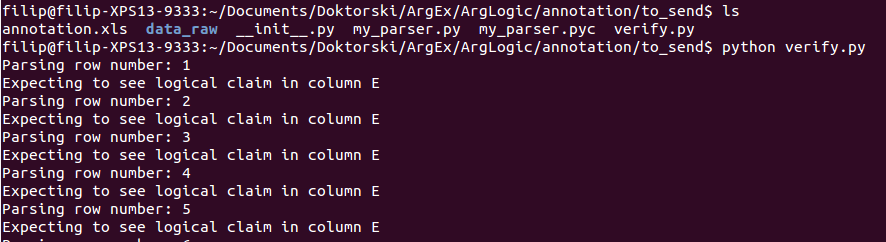
\includegraphics[scale=0.5]{struc_instructions_1.png}
	\caption{Expected output of running microstructure syntax check on entire file (\ref{item:excel}) mode}
	\label{fig:struc_instructions_all}
\end{figure}

\begin{figure}
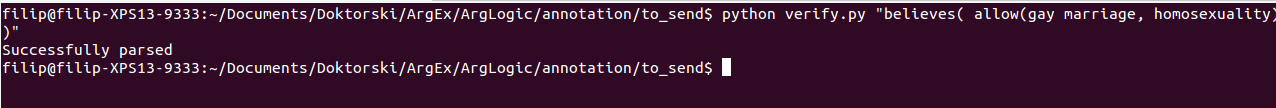
\includegraphics[scale=0.35]{struc_instructions_2.png}
	\caption{Expected output of running microstructure syntax check on a
	\label{fig:struc_instructions_2}
	single claim (\ref{item:single_claim} mode) }
\end{figure}

\noindent The script and your annotation is packaged into a zip available here. When you
unzip it, you should input your solutions in excel file \texttt{to\_send/annotation.xls}
To run it in \ref{item:excel} mode simply run \texttt{python verify.py} while
positioned in the \texttt{to\_send} directory using the command line (shown in
figure~\ref{fig:struc_instructions_all}) To run in \ref{item:single_claim}
mode, also position yourself in the \texttt{to\_send/} directory, but run as
shown in figure~\ref{fig:struc_instructions_2}.


\section{Claim segment annotation}
\label{sec:argseg_annotation}

Annotating claim segments from user comments splits the comment into claims. The
claims can be transformed into microstructures (as done to create the
microstructure dataset described in~\ref{item:microstructures_dataset}) or
formalized structures (as done to create the argument structure dataset
described in~\ref{item:structure_dataset}). Annotating segments involves
paraphrasing extracted segments to help streamline the annotation of segments
to structures. 

The task is to segment debate posts into claims. Each annotator gets a sheet in
a Google Sheets file with their name.  Column $C$ contains a user comment on
the topic of ``\textit{Should marijuana be legal}'' (MA).  The annotator needs
to carefully read the user comment, determine the stance of the comment along
with the explicit and implicit claims upon which the comment founds the
expressed stance. 

For each comment, the annotation involves:
\begin{enumerate}
\item extracting all argumentative segments of the comment as an atomic claim,
\item labeling the type of extracted segments, and
\item creating a paraphrase of the extracted segment.
\end{enumerate}
All argumentative segments should be copied to column $D$. 
Each extracted segment needs to be marked with an integer which denotes the
ordering of appearance in the post (segment $S1$, $S2$, $S3$, \dots)
All text belonging to segment $S1$ needs to be copied to column $D$, whereas
the original comment text needs to be edited to mark the segments belonging to 
the extracted segments. The beginning and end 
of the segment $Sx$ need to be marked with \texttt{<Sx>} and \texttt{</Sx>} respectively. 
Discontiguous segments are also allowed, they need to be marked with start and end tags
for each segment. Copying discontiguous segments is done by concatenating all 
instances in order of appearance. 
Column $E$ needs to contain the segment 
identifier ($S1$, $S2$, \dots). Please note that each start tag needs to be
paired with an end tag. 

\noindent Example 1: 

\begin{itemize}
  \item[] Comment: ``People are great, they have many virtues.''
  \item[] Segment $S1$: ``People are great''
  \item[] Segment $S2$: ``they have many virtues''
  \item[] Edited comment: ``\texttt{<S1>}People are great\texttt{</S1>},
  \texttt{<S2>}they have many virtues\texttt{</S2>}. ''
\end{itemize}

\noindent Example 2:
\begin{itemize}
\item[] Comment: ``People are smart and stupid.''
\item[] Segment $S1$: ``People are smart''
\item[] Segment $S2$: ``People are stupid''
\item[] Edited comment: ``\texttt{<S1><S2>}People are\texttt{</S2>} smart\texttt{</S1>}
and \texttt{<S2>}stupid\texttt{</S2>}''
\end{itemize}

\subsection*{Argumentative segment type}

The extracted segment needs to have a labelled segment type in column $F$ of
the Google sheets document. The segment needs to be classified according to two
taxonomies. First, the segment needs to be classified as either a 
\begin{enumerate}
\item fact --- statement that is true or untrue,
\item policy --- statement providing a solution or another series of questions in response to a fact,
\item value --- judgement, appraisal or evaluation. 
\end{enumerate}
Second, the segment needs to be labelled as either a 
\begin{enumerate}
\item assertion --- explicit statement or announcement or
\item rhetorical question --- question not expecting an answer. 
\end{enumerate}
More on facts, values and policies \citep{factvaluepolicy}.

\subsection*{Segment paraphrase annotation}

For each extracted segment, a paraphrase needs to be constructed. The paraphrase needs to
be assigned to column $G$ in spirit of the following principles:
\begin{itemize}
\item \textbf{Argumentativeness} -- Only argumentative text should be paraphrased; 
\item \textbf{Atomicity} -- A claim should convey a single thought; 
\item \textbf{Authority} -- Experts in claims from expert opinion should be made explicit in the paraphrase; 
\item \textbf{Brevity} -- Paraphrases should keep only the relevant argumentative content; 
\item \textbf{Canonicity} -- Canonical terms and phrases are preferred over idiomatic language;
\item \textbf{Contextuality} -- Claims should be paraphrased by considering their local and
topical context as well as their context;
\item \textbf{Declarativity} -- paraphrases should 
be in declarative form;
\item \textbf{Dereferencing} -- Pronouns and nominal  references
should be  resolved;  and
\item \textbf{Explicitness} -- Only explicitly stated
information should be paraphrased, and not whatever might be implied by the claim
\end{itemize}

\subsection*{Examples of segment annotation}

\begin{mydef}
By banning gay adoption, children in gay couple households have no legal status
should something happen to the parents, including death or serious illness.
The child cannot claim inheritances or other household assets in case of death.
If one parent dies, the second parent has no legal right to take custody or
care for the child.   A parent without legal right to a child cannot legally
register him/her for school.   Parents cannot put children on some health
insurance plans.   Parents cannot make medical decisions for the child.   * The
child has no claim to the social security or other insurance benefits of the
parent.   Gay couple parents without adoption rights do not benefit from the
generous tax deductions granted to heterosexual parents.
\end{mydef}

\noindent Extracted segments:
\begin{itemize}
\item[] \textbf{Segment1:} ``By banning gay adoption, children in gay couple
households have no legal status should something happen to the parents,
including death or serious illness.''
\item[] \textbf{Type}: Fact, assertion
\item[] \textbf{Paraphrase}: ``Children without a legal status are not
protected in case something happens to their parents''
\end{itemize}

\begin{itemize}[topsep=0.3cm]
\item[] \textbf{Segment2}: ``The child cannot claim inheritances or other household assets in case of death.''
\item[] \textbf{Type}: Fact, assertion
\item[] \textbf{Paraphrase}: ``Children without a legal status cannot claim
inheritance or other household assets in case of death.''
\end{itemize} 

\begin{itemize}[topsep=0.3cm]
\item[] \textbf{Segment3}: ``If one parent dies, the second parent has no legal
right to take custody or care for the child.''
\item[] \textbf{Type}: fact, assertion
\item[] \textbf{Paraphrase}: ``If one parent dies, the second parent has no legal
right to take custody or care for the child.'' (same)

\end{itemize}

\begin{itemize}[topsep=0.3cm]
\item[] \textbf{Segment4}: ``A parent without legal right to a child cannot
legally register him/her for school.''
\item[] \textbf{Type}: fact, assertion
\item[] \textbf{Paraphrase}: ``A parent without legal right to a child cannot
legally register him/her for school.'' (same)
\end{itemize}

\begin{itemize}[topsep=0.3cm]
\item[] \textbf{Segment5}: ``Parents cannot put children on some health insurance plans.''
\item[] \textbf{Type}: fact, assertion
\item[] \textbf{Paraphrase}: ``Parents cannot put children on some health insurance plans.'' (same)

\end{itemize}

\begin{itemize}[topsep=0.3cm]
\item[] \textbf{Segment6}: ``Parents cannot make medical decisions for the child.''
\item[] \textbf{Type}: fact, assertion
\item[] \textbf{Paraphrase}: ``Parents cannot make medical decisions for the child.''
\end{itemize}

\begin{itemize}[topsep=0.3cm]
\item[] \textbf{Segment7}: ``The child has no claim to the social security or
other insurance benefits of the parent''
\item[] \textbf{Type}: fact, assertion
\item[] \textbf{Paraphrase}: ``The child has no claim to the social security or
other insurance benefits of the parent''
\end{itemize}

\begin{itemize}[topsep=0.3cm]
\item[] \textbf{Segment8}: ``Gay couple parents without adoption rights do not
benefit from the generous tax deductions granted to heterosexual parents.''
\item[] \textbf{Type}: fact, assertion
\item[] \textbf{Paraphrase}: ``Unmarried gay parents cannot claim adoption rights
to benefit from tax deductions.''
\end{itemize}

\begin{mydef}
No it shouldnt be allowed. Marriage is when man and women get married. In the
Bible it says that its a sin for marrying your same gender and its a immoral
sin. Look at the animals they have one male and one female you dont see 2 male
horse with each other or any other animals. Look at the example animals make
learn from them.
\end{mydef}

\begin{itemize}[topsep=0.3cm]
\item[] \textbf{Segment1}: it shouldnt be allowed
\item[] \textbf{Type}: policy, assertion
\item[] \textbf{Paraphrase}: Gay marriage should not be allowed.
\end{itemize}

\begin{itemize}[topsep=0.3cm]
\item[] \textbf{Segment2}: Marriage is when man and women get married.
\item[] \textbf{Type}: fact, assertion
\item[] \textbf{Paraphrase}: Marriage is between a man and a woman.
\end{itemize}

\begin{itemize}[topsep=0.3cm]
\item[] \textbf{Segment3}: In the Bible it says that its a sin for marrying your same gender and its a immoral sin.
\item[] \textbf{Type}: fact, assertion
\item[] \textbf{Paraphrase}: According to the bible, same-sex marriage is immoral.
\end{itemize}

\begin{itemize}[topsep=0.3cm]
\item[] \textbf{Segment4}: Look at the animals they have one male and one female
\item[] \textbf{Type}: fact, assertion
\item[] \textbf{Paraphrase}: Animals of opposite sex pair up.
\end{itemize}

\begin{itemize}[topsep=0.3cm]
\item[] \textbf{Segment5}: you dont see 2 male horse with each other or any other animals
\item[] \textbf{Type}: fact, assertion
\item[] \textbf{Paraphrase}: Animals of same sex do not pair up.
\end{itemize}

\begin{itemize}[topsep=0.3cm]
\item[] \textbf{Segment6}: Look at the example animals make learn from them.
\item[] \textbf{Type}: policy, assertion
\item[] \textbf{Paraphrase}: We should learn from how animals behave.
\end{itemize}

\subsubsection*{Segment atomicity}

\begin{mydef}
I do not at all feel as God wants two men or two woman to be together, as he
has made each a man and a woman to combine and be together. However, it is our
constitutional right to make our own chices in America. What I believe should
be "exit only" is non of my business where people put things. As far as a legal
bond, we are considered "one nation under God" but , the goverment would make a
benifit from gay marriage, wether I a gree or not. Like I said we should have
the freedom to choose, we are Americans and our ancestors fought for our
freedom!!!!! Hey and I hope everyone is fighting to keep seatbelts a
choice,please keep fighting for our FREEDOM of choice!!!
\end{mydef}
This extracted segment expresses two separate ``thoughts''
\begin{itemize}
\item[] ``What I believe should be "exit only" is non of my business where people put
things.''
\end{itemize}
therefore it should be divided into two segments:
\begin{itemize}
\item[]  ``I believe should be "exit only"''
\item[] ``is non of my business where people put things''
\end{itemize}

\subsection*{Assuming too many implicit premises}

\begin{mydef}
I do not at all feel as God wants two men or two woman to be together, as he
has made each a man and a woman to combine and be together. However, it is our
constitutional right to make our own chices in America. What I believe should
be "exit only" is non of my business where people put things. As far as a legal
bond, we are considered "one nation under God" but , the goverment would make a
benifit from gay marriage, wether I a gree or not. Like I said we should have
the freedom to choose, we are Americans and our ancestors fought for our
freedom!!!!! Hey and I hope everyone is fighting to keep seatbelts a
choice,please keep fighting for our FREEDOM of choice!!!
\end{mydef}
The segment ``our ancestors fought for our freedom'' can be understood
such that the author believes that freedom refers to the freedom of choice.
This might be the case, but concluding so requires making assumptions based 
derived on implicit premises. 

\begin{itemize}
\item[] ``American ancestors fought for freedom to choose''
\end{itemize}
This paraphrase assumes ``freedom to choose''. But, the same segment can be
paraphrased not to include implicit knowledge and paraphrase in the following way 
(while also dereferencing the pronoun ``our'' to ``Americans''):
\begin{itemize}
\item[] ``Ancestors of current Americans fought for freedom of Americans.''
\end{itemize}

\subsection*{Reusing segment parts}

\begin{mydef}
As you say, "Marriage is something in particular." Its a legal union requiring
a license from a government office, not from a religious organization. That's
why gay people are fighting for "equal rights", not "equal rites."   For the
government to remain neutral on this issue, they need to stop denying gay
people the same rights as others to marry. As it is, the federal government is
anything but neutral. They deny over one thousand federal benefits to people
legally married in several states who happen to be of the same sex.
\end{mydef}
One candidate segment to extract would be:
\begin{itemize}
\item[] ``For the government to remain neutral on this issue, they need to stop
denying gay people the same rights as others to marry''
\end{itemize}
This segment actually contains three connected atomic segments (in paraphrased form):
\begin{itemize}
\item[] ``The government needs to remain neutral on this issue''
\item[] ``The government needs to stop denying gay people rights to marry''
\item[] ``Everyone but gay people have the rights to marry''
\end{itemize}


\begin{mydef}
This is the dictionary definition of marriage:   a.   the social institution
under which a man and woman establish their decision to live as husband and
wife by legal commitments, religious ceremonies, etc. Antonyms: separation.
b.   a similar institution involving partners of the same gender: gay marriage.
Antonyms: separation.   2.   the state, condition, or relationship of being
married; wedlock: a happy marriage. Synonyms: matrimony. Antonyms: single life,
bachelorhood, spinsterhood, singleness; separation.   3.   the legal or
religious ceremony that formalizes the decision of two people to live as a
married couple, including the accompanying social festivities: to officiate at
a marriage. Synonyms: nuptials, marriage ceremony, wedding. Antonyms: divorce,
annulment.   4.   a relationship in which two people have pledged themselves to
each other in the manner of a husband and wife, without legal sanction: trial
marriage.   5.   any close or intimate association or union: the marriage of
words and music in a hit song. Synonyms: blend, merger, unity, oneness;
alliance, confederation. Antonyms: separation, division, disunion, schism.
There is no mention of the reason for marriage being to Pro-create, the only
reason people should get married should be because they love each other and if
two Gay people love each other they should be allowed to marry. You can
Pro-create without getting married and I know many straight married people who
dont have Children they married because they loved each other not to have
children and Gay people should be allowed this right as well
\end{mydef}
Segment ``many straight married people who dont have Children they married
because they loved each other not to have children''
can be divided into three atomic segments:
\begin{itemize}
\item[] ``many straight married people who don't have Children''
\item[] ``many people married because they loved each other''
\item[] ``many people married not to have children''
\end{itemize}

\subsection*{Recognizing value segments}

Value segments often involve explicitly judging the value of an object.
Sometimes, the judgement can be made implicitly, but seeing explicit 
expressions should be preffered. For example: 
``People argue Gay marriage will lead to and allow
nontraditional families.'' is a factual statement, because 
the author expresses his views of public opinion. If the author expressed
his personal view like ``gay marriages lead to nontraditional families''
this could be considered a value statement, with the key part being
the word ``nontraditional'' which expresses negativity towards ``gay marriages''.
Whether there is a another view holder can influence the segment type. 
The segment ``The bible says Gay rights are immoral'' is considered a factual statement, 
whereas the segment ``Gay rights are immoral'' is considered to be a 
value segment since the segment is attributed to the author. 


\section{Prominent Claim Identification Annotation}
\label{sec:argrec_annotation}

Prominent claim identification is the task of recognizing which (from a set of
predefined) prominent claims is mentioned in a target comment and how. The goal
of the task is to label prominent claim-comment pairs with a label:
\begin{itemize}
	\item \textbf{A} -- explicitly attacks the prominent claim
	\item \textbf{a} -- vaguely/implicitly attacks the prominent claim
	\item \textbf{N} -- makes no use of the prominent claim
	\item \textbf{s} -- vaguely/implicitly supports the prominent claim
	\item \textbf{S} -- explicitly supports the prominent claim
\end{itemize}
Labeling the dataset according the guidelines below
produced the \ComArg dataset (described in section~\ref{sec:comarg}.

\subsection*{Annotation Guidelines}

There is an online discussion about ``gay rights''. The topic is ``SHOULD GAY
PEOPLE BE ALLOWED TO MARRY?''. Users post comments on the discussion forum,
which express opinions that are either for or against gay marriages. For
example: COMMENT: ``Gay people shouldn’t marry because they can’t have
children.''
In these discussions, users often refer to certain well-established arguments .
For example, typical arguments are:
\begin{itemize}
\item ARGUMENT 1: ``All people should be treated equally.''
\item ARGUMENT 2: ``Marriage should be between two believers who can produce godly offspring.''
\item ARGUMENT 3: ``Marriage is about more than procreation, therefore gay couples should not be denied the right to marry due to their biology.''
\end{itemize}

\noindent Your task is to detect WHICH arguments are used in a comment and HOW. You will
be presented with three arguments for each comment. For each argument, there
will be five check boxes, numbered 1 (DENIED) through 5 (APPROVED). 

\noindent For each argument, you need to do the following:
\begin{itemize}
\item if the comment directly denies the argument, check 1 (DENIED).
\item if the comment does not refer to the argument, check 3 (NOT MENTIONED)
\item if the comment approves the argument to make its point, check 5 (APPROVED).
\end{itemize}

\noindent You might feel that the comment approves or denies the argument, but you're not
completely certain. If you think that the argument is indirectly or partially
denied, check option 2, which is the option between DENIED and NOT MENTIONED.
Conversely, if you think that the argument is indirectly or partially approved,
check option 4, which is the option between NOT MENTIONED and APPROVED.
Note that it will often be the case that an argument is not mentioned.

Also note that if a comment and an argument express a different opinion, it
does not automatically mean that the argument is denied. For example, a comment
``Marriage is a religious institution, and the major world religions frown upon
homosexuality'' does not deny the argument ``Gay couples should be able to take
advantage of the fiscal and legal benefits of marriage''. Here, the comment and
the argument do express different opinions over the issue, but the argument
itself is not mentioned in the comment.

Consider again the example above. To detect whether and how ARGUMENTS 1-3 are
used in COMMENT, think in the following way.
In case of ARGUMENT 1: ``All people should be treated equally.''

\begin{enumerate}
\item    ARGUMENT 1 refers to human equality
\item    COMMENT does NOT refer to human equality
\item    Therefore, check option 3 (NOT MENTIONED) for ARGUMENT 1.
\end{enumerate}

\noindent In case of ARGUMENT 2: ``Marriage should be between two believers who can
produce godly offspring.''

\begin{enumerate}
\item ARGUMENT 2 implies that having children is a necessary condition for
marriage
\item COMMENT states that gay people shouldn’t marry because they cannot have
children, implying that having children is a necessary condition for marriage
\item BOTH claims are about having children and make the same point
\item therefore, COMMENT supports ARGUMENT 2
\item check option 5 (APPROVED)
\end{enumerate}

\noindent In case of ARGUMENT 3: ``Marriage is about more than procreation, therefore gay
couples should not be denied the right to marry due to their biology.''

\begin{enumerate}
\item ARGUMENT 3 implies that having children is not a necessary condition for marriage
\item COMMENT states that gay people shouldn’t marry because they cannot have children, implying that having children is a necessary condition for marriage
\item BOTH claims are about ``having children'', but COMMENT states the opposite of ARGUMENT 3
\item therefore, COMMENT denies ARGUMENT 3
\item check option 1 (DENIED)
\end{enumerate}


\section{Implicit claim annotation}
\label{app:sec:argpremises_annotation}

\subsection*{Annotation guidelines}

%This produced the argpremises dataset similarities in the (\ref{item:argpremises}).

IMPORTANT: This is essentially a reading comprehension task. While we
appreciate your opinion on this topic, this task is about analyzing OTHER
PEOPLE'S OPINIONS, not expressing your own. This is not an online survey.

\noindent There is an online discussion on marijuana legalization. The topic is: ``SHOULD
MARIJUANA BE LEGALIZED?''. You have to be familiar with of the issue: You can
get basic information about the topic 
in the footnotes\footnote{\url{http://medicalmarijuana.procon.org/}}\footnote{
\burl{http://idebate.org/debatabase/debates/health/addiction/
house-believes-cannabis-should-be-legalised}
}
Your goal is to identify whether the two sentences offered are talking about
the same thing. Please rate the SIMILARITY LEVEL for each pair of sentences:
\begin{itemize}
\item 6: very similar
\item 5 or 4: somewhat similar
\item 3 or 2: somewhat dissimilar
\item 1: not similar
\end{itemize}

\noindent Example one:
\begin{table}[h!]
\begin{tabular}{|@{\ }r@{\ \  }p{0.72\columnwidth}|}
\hline
\textbf{Sentence 1:} & \emph{Marijuana does not cause any damage to our bodies}\\
\textbf{Sentence 2:} & \emph{Consuming pot never hurt anyone}\\
\textbf{Similarity level} & 6 \\
\hline
\end{tabular}
\end{table}
\pagebreak
%\caption{User claim, the matching main claim, and the implicit premises filling the gap.}

\noindent Example two:
\begin{table}[h!]
\begin{tabular}{|@{\ }r@{\ \  }p{0.72\columnwidth}|}
\hline
\textbf{Sentence 1:} & \emph{If legalized, people will use marijuana and other drugs more}\\
\textbf{Sentence 2:} & \emph{Marijuana can be used as medicine because it showed positive effects}\\
\textbf{Similarity level} & 1 \\
\hline
\end{tabular}
\end{table}

\noindent Example three:
\begin{table}[h!]
\begin{tabular}{|@{\ }r@{\ \  }p{0.72\columnwidth}|}
\hline
\textbf{Sentence 1:} & \emph{A large portion of modern music an art has been inspired by marijuana}\\
\textbf{Sentence 2:} & \emph{Used as a medicine for its positive effects}\\
\textbf{Similarity level} & 4 \\
\hline
\end{tabular}
\end{table}


\section{Claim formalization annotation}
\label{sec:formalization_annotation}

This produced the \ref{item:structure_dataset}

\subsection{Cheat sheet}

\textbf{Task}: Transform natural language claims into logical form. Logical form needs to have:
\begin{itemize}
\item Domain individuals 
\item Claim relation
\item Modality
\item (Opinion holder)
\end{itemize}

\noindent \textbf{Domain individual} \\
Find appropriate individuals mentioned in the claim (i.e. \textit{marijuana consumers},
\textit{brain damage}, \textit{legalized tobacco}, \textit{heroin}, \textit{mafia selling marijuana}) \\

\noindent \textbf{Claim relations} \\

\begin{tabular}{| l |  p{9cm} | p{3cm}| }
\toprule
\textbf{Promotes} & 
\makecell[cc]{
\texttt{has\_antecedent + domain\_individual} \\
\texttt{promotes + domain\_individual}
}
& 
fosters, brings about, leads, forces, advances \\
\midrule
\textbf{Implies} &
\makecell[cc]{
\texttt{has\_antecedent + domain\_individual} \\
\texttt{implies + domain\_individual}
}
&
if .. then .. is \\
\midrule
\textbf{Causes} & 
\makecell[cc]{
\texttt{has\_antecedent + domain\_individual} \\
\texttt{causes + domain\_individual}
}
& causes \\
\midrule
\textbf{Suppresses} & 
\makecell[cc]{
\texttt{has\_antecedent + domain\_individual} \\
\texttt{suppresses + domain\_individual}
} &
inhibits, stops, decreases \\
\midrule
\textbf{Contradicts} & 
\makecell[cc]{
\texttt{has\_antecedent + domain\_individual} \\
\texttt{contradicts + domain\_individual}
} &
if .. then not .., is .. not a \\
\midrule
\textbf{Does not cause} &
\makecell[cc]{
\texttt{has\_antecedent + domain\_individual} \\
\texttt{does\_not\_cause + domain\_individual}
} &
causes not, does not cause \\
\midrule
\textbf{Declaration} &
\makecell[cc]{
\texttt{has\_declaration + domain\_individual}
} &
defines, exists \\
\midrule
\textbf{Comparison} &
\makecell[cc]{
\texttt{comparison\_greater + domain\_individual} \\
\texttt{comparison\_less + domain\_individual} \\
	(\texttt{comparison\_property + domain\_individual})
} &
less than, more than, greater than \\
\bottomrule
\end{tabular}
\\

\textbf{Modality} $\Rightarrow$ \texttt{has\_modality + fact/good\_value/bad\_value/policy} \\

\textbf{Opinion holder} $\Rightarrow$ \texttt{has\_opinion\_holder + domain\_individual} \\

\subsection{Examples cheat sheet}

\noindent \textbf{Promotes} \\
\begin{tabular}{p{8cm} p{8cm}}
Marijuana legalization increases crime rates. & \texttt{legalized\_marijuana promotes crime} \\
Smoking marijuana makes people happy. & \texttt{marijuana\_consumer promotes happiness}
\end{tabular}

\noindent \textbf{Implies} \\
\begin{tabular}{p{8cm} p{8cm}}
Marijuana is a drug. & \texttt{marijuana implies any\_drug} \\
	If we legalize marijuana, the government will earn money.  &\texttt{legalized\_marijuana implies government\_making\_money}
\end{tabular}
 
\noindent \textbf{Causes} \\
\begin{tabular}{p{8cm} p{8cm}}
	Marijuana consumption causes death. & \texttt{marijuana\_consumer causes death}  \\
	Marijuana legalization made government each money. & \texttt{legalized\_marijuana causes government\_earning\_money}\\
	Marijuana use alters the mind. & \texttt{marijuana\_consumer causes mind\_influential. }
\end{tabular}

\noindent \textbf{Suppresses}  \\
\begin{tabular}{p{8cm} p{8cm}}
	Legalizing marijuana hurts the balance of the economy. & \texttt{legalized\_marijuana suppresses government\_making\_money} \\
	Consuming marijuana decreases aggressive behavior. & \texttt{marijuana\_consumer suppresses aggressive\_behavior} \\
	Legalizing marijuana lowers the number of consumers. & \texttt{legalized\_marijuana supppresses marijuana\_consumer}
\end{tabular}

\noindent \textbf{Contradicts} be careful with double negation! \\
\begin{tabular}{p{8cm} p{8cm}}
	If legalization of marijuana happens, there will be no crime. & \texttt{legalized\_marjuana contradicts crime} \\
	Tobacco is not a plant. & \texttt{tobacco contradicts any\_plant}
\end{tabular}

\noindent \textbf{Does not cause} be careful with double negation! \\
\begin{tabular}{p{8cm} p{8cm}}
	Consuming marijuana does not cause death. & \texttt{marijuana\_consumer does\_not\_cause death} \\
	Legalizing marijuana never helped the government economy. & \texttt{legalized\_marijuana does\_not\_cause government\_making\_money}
\end{tabular}

\noindent \textbf{Declaration} \\
\begin{tabular}{p{8cm} p{8cm}}
	Marijuana is widely used. & \texttt{declaration marijuana\_consumer}  \\
	Marijuana should not be legalized. & \texttt{declaration illegal\_marijuana} \\
	I don’t consume marijuana.  & \texttt{declaration non\_marijuana\_consumer}
\end{tabular}

\noindent \textbf{Comparison} \\
\begin{tabular}{p{8cm} p{8cm}}
	Alcohol is more stimulative than marijuana. & \texttt{comparison\_more alcohol + comparison\_less marijuana + comparison\_property stimulative\_behavior}\\
	Heroin is worse than marijuana. & \texttt{comparison\_more herion + comparison\_less marijuana}
\end{tabular}

\subsection{Introduction}

The goal is to transform natural language claims to logical form given claims
and rules for annotation of logical form. This document explains the rules for
annotation. For example, given a claim ``The government will make a huge profit
from legalizing marijuana'' made on the topic of \textit{Drug legalization} by an author
named \textit{Fred}, we wish to transform it into logical form which would be: \\

\noindent \texttt{
author(Fred) \^{} has\_claim(Fred, c) \^{} has\_modality(c, fact) 
\^{} has\_antecedent(c, marijuana\_legalization) 
\^{} implies(c, government\_profit)
} \\

\noindent The logical form and its rules are defined by the ontology that has been
pre-created for each topic. To annotate data, you will need to use a tool named
\textit{Protege} to load the ontology. 
The outline of the annotation is: 
\begin{enumerate}
\item Open Protege and load pre-created ontology
\item Read and understand the claim individual and its entire post.  
\item Tranform the claim individual to logical form in Protege by adding properties to the claim
individual. 
\end{enumerate}

\subsubsection{Setup}

To annotate data you will need:
\begin{enumerate}
\item Download and install Protege 5, an ontology tool
\item Load provided ontology in Protege 5
\end{enumerate}
Download and install the desktop version of Protege 5. Links for Windows instructions:
\begin{itemize}
\item \url{https://protege.stanford.edu/products.php#desktop-protege}
\item \url{https://protegewiki.stanford.edu/wiki/Instal_Protege5_Win}.
\end{itemize}

\subsection{Annotation steps}

All the annotation will be done in the individuals tab of Protege. 
We discern between \textbf{domain} and \textbf{claim individuals}. 
\textbf{Domain individuals} are domain-specific as they
were mentioned previously in the debate, \textbf{claim individuals} are individuals
representing the logical form of natural language claims. 
You need to formalize natural language claims 
by recognizing claim relation and domain individuals
used to add properties to a \textbf{claim individual}. In total, you need to do \textbf{four}
steps to annotate a natural language claim:
\begin{enumerate}[label=\textbf{Step \arabic*.}, leftmargin=2cm]
\item select which domain individuals from a predefined list are used in the claim,
\item recognize which claim relation is used in the claim individual, 
\item which modality was used for the claim (\texttt{fact/value/policy}), and 
\item identify the claim opinion holder. 
\end{enumerate}


\subsubsection{Step 1: Choosing domain individuals}

We offer a list of \textbf{domain individuals} to choose from beforehand (loaded with
the ontology). We consider domain individuals well-established topics in the
debate as the authors mostly agree on them. Examples are: \textit{mafia selling
marijuana, marijuana tax, marijuana legalization, alcohol, science, obesity} \dots
They are usually nouns with adverbs. Some domain individuals are very similar
and it’s important to find the appropriate, most specific one, since you will
be offered both \textit{marijuana} and \textit{legalized marijuana}, you need to recognize which
domain individual is most appropriate given the claim. In case you don’t see an
appropriate domain individual, add a comment to the claim. We expect this to be
the case in ~15\% of the time. The goal of using domain individuals is to
transform sentences into logical with a minimal loss in meaning. Sometimes, you
will need to transform sentences from active to passive, or make verb nouns. 
For example, even though \textit{marijuana legalization}, \textit{marijuana legalizing} and
\textit{legalized marijuana} are three different concepts, we consider them the \underline{same
domain individual}. 

\subsubsection{Step 2.2: Recognizing claim relations}

Claim relations are usually, but not always, indicated by the main verb or the
conjunction in the claim. We’ve noticed four basic different claim relations
with four more subrelations (we highlight subrelations in the table with
$\rightarrow$). In the table below, we list the claim relations, possible
indicators that might hint the claim relation, the pattern in which the claim
relation might appear in natural language with respect to domain individuals
(A, B, C represent any domain individual) and an example of a natural language
claim containing the claim relation. 

\begin{tabular}{| l | p{3.5cm} | p{3cm} | p{5cm}| }
\toprule
\cellcolor{gray!25} Claim relation & \cellcolor{gray!25}Indicators &
\cellcolor{gray!25}Pattern & \cellcolor{gray!25}Example \\
\midrule
	\textbf{Promotes} & 
	Promotes, fosters, brings about, leads, forces, advances & 
	\textbf{A} promotes \textbf{B} &
\textit{Marijuana legalization improves health} \\
\midrule
	$\rightarrow$ \textbf{Implies} & 
	Implies, entails, if \dots then, is &
	\textbf{A} implies \textbf{B} &
\textit{If marijuana is legal, the crime rate will rise. } \\
\midrule
	$\rightarrow$ \textbf{Causes} &
	Causes &
	\textbf{A} causes \textbf{B} &
\textit{Marijuana legalization causes an increase in crime rate.} \\
\midrule
	\textbf{Suppresses} &
	Similar to promotes, but negative inhibitor &
	\textbf{A} suppresses \textbf{B} &
	\textit{ Marijuana hurts health. } \\
	\midrule
	$\rightarrow$ \textbf{Contradicts} &
	Does not imply, if \dots then not, is not &
	\textbf{A} implies not \textbf{B} &
\textit{If marijuana is legal, no crime will happen. } \\
\midrule
	$\rightarrow$ \textbf{Does not cause} &
	Does not cause &
	\textbf{A} does not cause \textbf{B} &
\textit{Growing marijuana at home does not stop mafia selling marijuana. } \\
\midrule
	\textbf{Declaration} &
	defines, exists &
	\textbf{A} &
\textit{Legalized marijuana exists.} \\
\midrule
	\textbf{Comparison} & 
	Is more than, has more, does less &
	\textbf{A} is more than \textbf{B} by criteria \textbf{C} &
\textit{Marijuana is less addictive than alcohol} \\
\bottomrule
\end{tabular}

In the case of promotes, its subrelation are implies and causes. Contradicts
and does not cause are subrelation of suppresses. Subrelation are \textbf{more specific}
than a claim relation meaning, if there is an implies relation, it is also a
promotes, and, if there is a contradiction or does not cause relation, it is
also a suppresses. 

\subsubsection{Step 2.2 Annotation claim relations}

Now that you’ve recognized the claim relation and domain individuals, you need
to add properties to a \textbf{claim individual}. We now explain how to annotate for
each of the four claim relations and subrelations. Promotes and suppresses are
binary (two domain individuals), declaration is unary (single domain
individuals), and comparison is ternary (three domain individuals). 

\subsubsection{Promotes}

For promotes you can choose between three options (one claim relation and two
claim subrelations):
\begin{itemize}
\item Promotes (most general) $\Rightarrow$ Promotes 
\item Implies $\Rightarrow$ Implies
\item Cause $\Rightarrow$ Causes
\end{itemize}
Implies corresponds to someone saying in the form of implication (if A then B,
A is B). Causes is when people say that one thing causes another (A causes B).
When you’re \textbf{unsure} which one to choose, but see a general pattern of (A
promotes B, A stimulates B \dots) choose promotes as a more general term.
In the case of promotes (and suppresses) you also need to specify the
\texttt{has\_antecedent} property (domain individual A in A promotes B). An example for
the claim tobacco implies cancer is below is in figure~\ref{fig:promotes_example}

\begin{figure}
	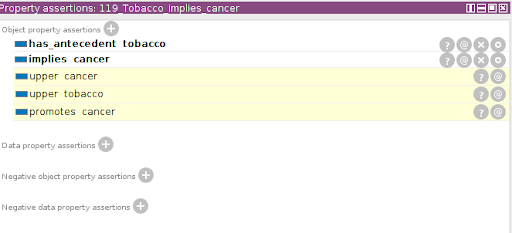
\includegraphics{promotes.png}
	\caption{Example of correct annotation for the \texttt{promotes} relation in Protege}
\label{fig:promotes_example}
\end{figure}

\subsubsection{Suppresses}

Suppresses is the \textbf{opposite} of promotes. Everything valid for promotes
also applies to suppresses, but instead of causes you have
\texttt{does\_not\_cause} and instead of \texttt{implies} you have \texttt{contradicts}.

\paragraph{Declaration}

A declaration is simply a claim stating a domain concept either exists, should
be done or is good/bad. The claim \textit{mafia sells marijuana} is annotated by adding
the \texttt{has\_declaration} with the appropriate domain individual (as seen in figure
\ref{fig:declaration_example}). 

\begin{figure}
	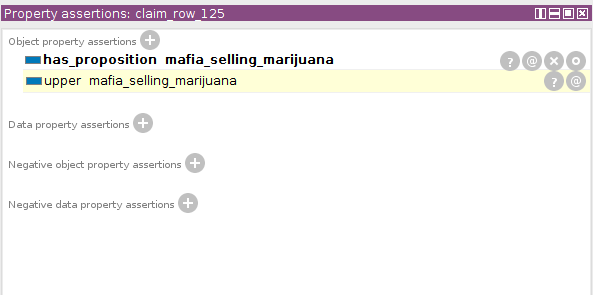
\includegraphics[scale=0.8]{has_declaration.png}
	\caption{Example of correct annotation for the \texttt{has\_declaration} relation in Protege}
\label{fig:declaration_example}
\end{figure}

\subsubsection{Comparison}

Comparisons in debates arise when someone compares two domain individuals,
usually (but not always) by saying one is better according to some feature
(which is a domain individual). The comparison pattern is A is more than B by
C. The domain individual for more is annotated with
\texttt{comparison\_greater}, less is ith \texttt{comparison\_less} and the
optional property of comparison is annotated with
\texttt{comparison\_property}. If there is no property, but an expression like
A is better than B is made, we don’t annotate \texttt{comparison\_property}.
The claim \textit{Alcohol is more influential on the mind than marijuana} is an
example annotated in the figure~\ref{fig:comparison_example}.

\begin{figure}
	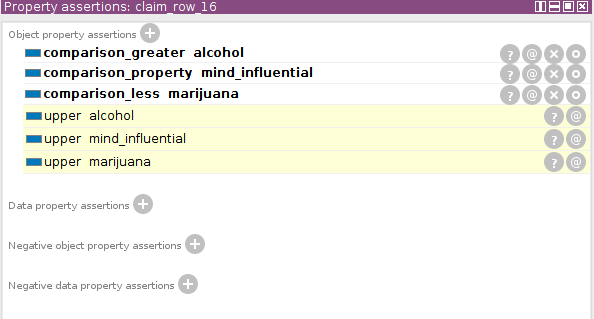
\includegraphics[scale=0.7]{comparison.png}
	\caption{Example of correct annotation for the \texttt{comparison} relation in Protege}
	\label{fig:comparison_example}
\end{figure}

\subsubsection{Step 2.3 Negation}

If you think you need to negate the selected relation, for example in the
sentence: \textit{Marijuana legalization does not promote crime} the author explicitly
states that one domain individual \textbf{does not promote} another. As not promoting \textbf{is
not always} the same as suppresses, we allow you to add negation to any
relation to reflect that. To add negation, simply select ``Negative object
property assertions'' instead of ``Object property assertions'' along with your
relation. Example on the figure \ref{fig:negation_example}. Be \underline{very careful}
when opting for negation, especially with double negation.

\begin{figure}
	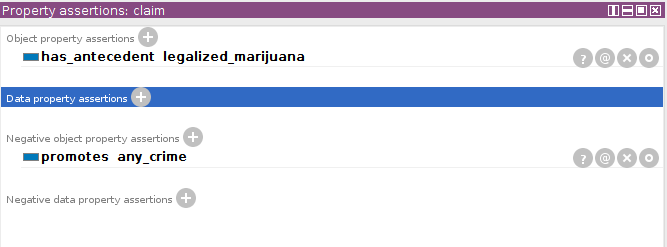
\includegraphics[scale=0.7]{negation.png}
	\caption{Example of correct annotation for negation in Protege}
	\label{fig:negation_example}
\end{figure}

\subsubsection{Step 3 Selecting modality}

We recognize that claims are made in a certain modality (way which they were
expressed with) and discern between:

\begin{itemize}
\item \textbf{Facts}:  believes/argues/thinks that claim C is true (example:
	\textit{Marijuana is legal})
\item \textbf{Policies}: A believes/argues/thinks C should be true in the
	future or should remain true  (example: \textit{Marijuana should be legal}) 
\item \textbf{Value judgement}: A believes/argues/thinks C is morally/ethically
	right or wrong
	\begin{itemize}
	\item Judging of good (example: \textit{Marijuana is great})
	\item Judging of bad (example: \textit{Marijuana sucks})
	\end{itemize}
\end{itemize}
After recognizing the modality, we need to add a property of \texttt{has\_modality} which
can be one of \texttt{fact, policy, good\_value, bad\_value}. 

\subsubsection{Opinion holder}

If the author mentions that his claim is made by someone else, we need to
annotate this information. For example, the following two claims are not made
by the same opinion holder:

\begin{enumerate}
\item Science says marijuana kills people
\item I think marijuana kills people
\end{enumerate}
For the first claim we need to add a property of \texttt{has\_opinion\_holder} to the
claim individual. The opinion holder can be any \textbf{domain individual}. In this
case, the opinion holder is science in claim 1). For claim 2), we don't need to
add a property \texttt{has\_opinion\_holder}, since the default opinion holder is the
author. 

\subsubsection{Step 5 Claim annotation comments}

This is an optional step if you can't annotate the claim for some reason. You
need to annotate the claim individual with a comment if you can't get its
logical form. \textbf{All} claim individuals \textbf{should be annotated with logical form or
commented on}. Adding a comment is done by clicking '+' in the \texttt{Annotations} and
selecting \texttt{rdfs:comment} for a specific claim. If you're missing a domain
individual (see step 1), you can simply write \textit{missing domain individual X},
where X is the domain individual you deem required to get a logical form. 
Figure~\ref{fig:comment_example} shows 
a claim individual, upper pane shows the annotations part where
you can add your comment. 

\begin{figure}
	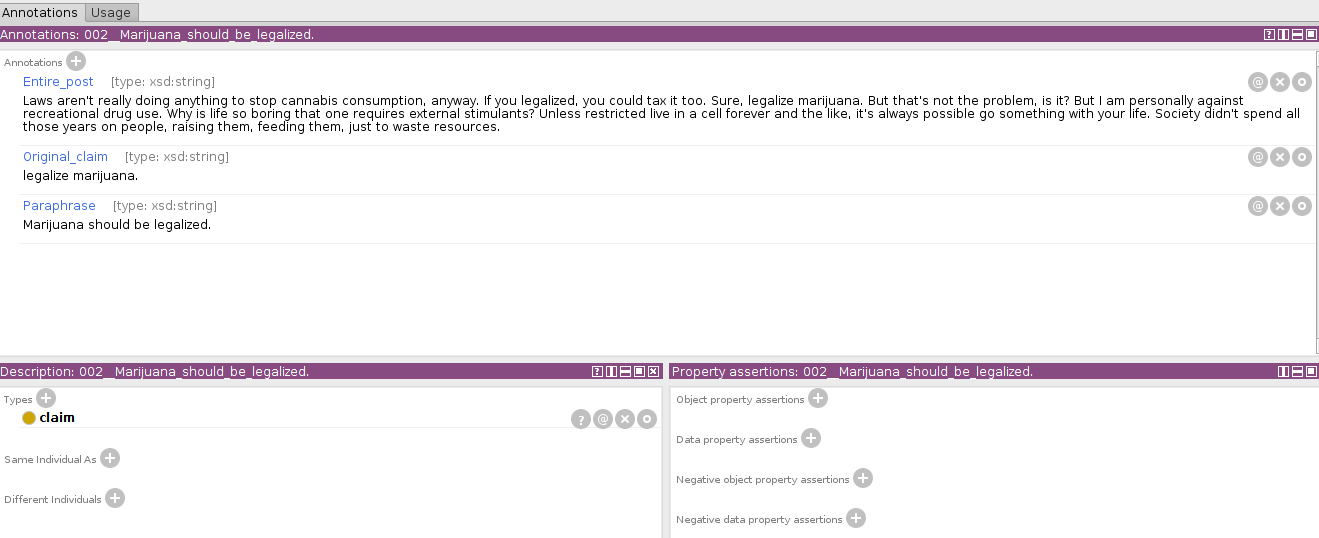
\includegraphics[scale=0.35]{comment.png}
	\caption{Example of correct annotation for adding a comment in Protege}
	\label{fig:comment_example}
\end{figure}

\subsection{Annotation Examples}

\begin{mydef}
 \textit{Marijuana legalization will increase crime rate. }
\end{mydef}

\begin{enumerate}[label=\textbf{Step \arabic*.}, leftmargin=2cm, itemsep=0.5cm]
\item You need to see which domain individuals are mentioned in the claim.
\textit{Marijuana legalization} and \textit{crime rate} are candidate noun phrases which
might be a good place to start. 
\item You see there is a will increase verb and you consult with table in step
2.1. You can narrow down the choice between promotes, implies and
causes as one thing supports another (\textit{marijuana legalization}
and \textit{crime rate}).  
\item To get the modality expressed you can work by elimination. Is there an
estimation if this is good or bad (if so, then value). Is there a
proposal of something that should be done? (if so, policy).
		Otherwise, it’s a factual information. 
\item There seems to be no mention of who is making the claim, so that should
	be the author. 
\end{enumerate}

\noindent Protege steps. 
\begin{enumerate}
\item Select the claim in Protege
\item Enter ``Object property assertions'' depending on the claim pattern identified 
\item Enter: \texttt{has\_antecedent} \texttt{legalized\_marijuana} (Step 1 \& 2)
\item Enter: \texttt{promotes any\_crime} (Step 1 \& 2)
\item Enter: \texttt{has\_modality fact} (Step 3)
\end{enumerate}

\begin{mydef}
Growing marijuana does not make mafia stop selling marijuana.
\end{mydef}

\begin{enumerate}[label=\textbf{Step \arabic*.}, leftmargin=2cm, itemsep=0.5cm]
\item Here we start from domain individuals. Marijuana and mafia related domain
	individuals seem appropriate. Looking into possible options there is a
		domain individual of \texttt{marijuana\_farmer} which seems to be the
		closest to growing marijuana. For mafia, the most similar
		individual seems \texttt{mafia not selling marijuana}
\item  Focusing on the main verb phrase ``does not make'', we can notice the
	pattern A does not cause B, hence we pick \texttt{does\_not\_cause}. We omit the
		rest of the steps as they are similar to example 1. 
\end{enumerate}
Protege steps
\begin{enumerate}
\item Select the claim in Protege
\item Enter “Object property assertions”
\item Enter \texttt{has\_antecedent marijuana\_farmer} (Step 1\&2)
\item Enter \texttt{does\_not\_cause mafia\_not\_selling\_marijuana} (Step 1\&2)
\item Enter \texttt{has\_modality fact} (Step 3)
\end{enumerate}




\end{appendices}

%%%%%%%%%%%%%%%%%%%%%%%%%%%%%%%%%%%%%%%%%%%%%%%%%%%%%%%%%%%%%%%%%%%%%%%%%%%
\backmatter

%%%%%%%%%%%%%%%%%%%%%%% LITERATURA / BIBLIOGRAPHY %%%%%%%%%%%%%%%%%%%%%%%%%
% bibliography style file is modified IEEEtran.bst file,
% changed to suit FER's literature style
\addcontentsline{toc}{chapter}{Literatura}
\bibliographystyle{IEEEtranFER} 
\bibliography{bibliography}
% \bibliography{eg_biblio}



%%%%%%%%%%%%%%%%%%%%%%% POPIS OZNAKA / NOMENCLATURE %%%%%%%%%%%%%%%%%%%%%%%
% notation and list of symbols if needed
%\printnomenclature

%%%%%%%%%%%%%%%%%%%%%%%%%%% KAZALO POJMOVA / INDEX %%%%%%%%%%%%%%%%%%%%%%%%
% optional index
%\printindex

%%%%%%%%%%%%%%%%%%%%%%%%%%%%%%%%% LOF %%%%%%%%%%%%%%%%%%%%%%%%%%%%%%%%%%%%%
% insert optional list of figures
% \listoffigures
%\cleardoublepage % start new page
%%%%%%%%%%%%%%%%%%%%%%%%%%%%%%%%% LOT %%%%%%%%%%%%%%%%%%%%%%%%%%%%%%%%%%%%%
% insert optional list of tables
% \listoftables
%\cleardoublepage % start new page

%%%%%%%%%%%%%%%%%%%%%%%%% ŽIVOTOPIS / BIOGRAPHY %%%%%%%%%%%%%%%%%%%%%%%%%%%
\renewcommand{\leftmark}{Životopis}
\chapter*{Životopis}
\addcontentsline{toc}{chapter}{Životopis}

% Životopis autora doktorskog rada treba biti napisan u trećem licu jednine, a
% opsegom ne smije prelaziti 1500 znakova (uključujući razmake).

Filip Boltužić rođen je 19. rujna 1988. u Sisku u Hrvatskoj. Prediplomski
studij računarstva završio je 2010. godine na Fakultetu elektrotehnike i računarstva
Sveučilišta u Zagrebu s temom ``Primjena algoritma kolonije pčela na kombinatoričke probleme''. 
Na istome je fakultetu završio i diplomski studij računarstva
(smjer računarska znanost) s temom ``Tehnike prikupljanja i vizualizacije
velikih skupova podataka''. 

Od listopada 2012. do travnja 2014. zaposlen je u odjelu Poslovne inteligencije 
Zagrebačke banke Unicreditgroup d.o.o. kao 
mlađi analitičar. Od srpnja 2014. do rujna 2017. zaposlen je 
u Amazon Web Services Ireland Ltd. kao razvojni inženjer. 
Od siječnja 2018. do siječnja 2020. 
zaposlen je na Zavodu za elektroniku, mikroelektroniku, računalne
i inteligentne sustave Fakulteta elektrotehnike i računarstva  
na projektu Uspostava integralnog sustava za 
upravljanje službenom dokumentacijom Republike Hrvatske kao voditelj razvoja.

Njegovi istraživački interesi obuhvaćaju područje obrade prirodnog jezika,
pretraživanja informacija i strojnog učenja. 
Član je strukovne udruge ACL (Association for Computational Linguistics). 
Govori engleski jezik.

\section*{Popis objavljenih djela}

% \subsection*{Rad u časopisima}
% 
% % TODO make enumerate
% 
% \begin{itemize}
% % \item Prezime1, InicijalImena1., Prezime2, InicijalImena2., Prezime3,
% % 	InicijalImena3., ``Naslov članka'', Naziv časopisa, Vol. X, No. Y (ili
% % 		Issue Y), mjesec i godina, str. A-B.
% \item Boltužić, F., Di Buono, M.P., Šnajder, J., Semantic-web journal
% \end{itemize}

\subsection*{Radovi na međunarodnim znanstvenim skupovima}

% TODO make enumerate
\begin{itemize}

\item Brassard, A., Kuculo, T., Boltužić, F., Šnajder, J., 
``TakeLab at SemEval-2018 Task12: Argument Reasoning Comprehension with Skip-Thought Vectors'',
12th International Workshop on Semantic Evaluation (SemEval-2018),
siječanj 2018., str. 1133-1136
\item Boltužić, F., Šnajder, J., 
``Toward Stance Classification Based on Claim Microstructures'',
Proceedings of the 8th Workshop on Computational Approaches to Subjectivity,
Sentiment and Social Media Analysis (WASSA) in conjunction with 
Conference on Empirical Methods in Natural Language Processing (EMNLP 2017),
rujan 2017., str. 74-80
\item Boltužić, F., Šnajder, J., 
``Fill the Gap! Analyzing Implicit Premises between Claims from Online Debates'',
Proceedings of the 3rd Workshop on Argument Mining in conjunction 
with 54th Annual Meeting of the Association for Computational Linguistics (ACL 2016),
lipanj 2016., str. 124-133
\item Tutek M., Sekulić I., Gombar P., Paljak I., Čulinović F., Boltužić
F., Karan M., Alagić D., and Šnajder J., ``TakeLab at
SemEval-2016 Task 6: Stance Classification in Tweets Using a
Genetic Algorithm Based Ensemble.'', Tenth International
Workshop on Semantic Evaluation (SemEval), lipanj 2016., str. 464–468
\item Boltužić, F., Šnajder, J.,
``Identifying prominent arguments in online debates using semantic textual similarity.'',
Proceedings of the 2nd Workshop on Argumentation Mining in conjunction
with 17th Annual Conference of the North American Chapter of the Association for
Computational Linguistics: Human Language Technologies
(NAACL-HLT 2019), lipanj 2015., str. 110-115
\item Boltužić, F., Šnajder, J., 
``Back up your Stance: Recognizing Arguments in Online Discussions'', 
Proceedings of the First Workshop on Argumentation Mining 
in conjunction with 52st Annual Meeting of the Association for Computational Linguistics (ACL 2014),
lipanj 2014., str. 49-58
\end{itemize}

\renewcommand{\leftmark}{Biography}
\chapter*{Biography}
\addcontentsline{toc}{chapter}{Biography}

Filip Boltužić was born on September 19, 1988 in Sisak, Croatia. 
He received his B.Sc. in Computing from the University of Zagreb, 
Faculty of Electrical Engineering and Computing in 2010 (thesis title:
``Application of the Bee Colony Optimization algorithm for combinatiorial problems'')
and M.Sc. in Computer Science from the same university in 2012 (thesis title:
``Online Analytical Processing Methods and Data Visualization'')

From October 2012 to April 2014 he was employed as a business analyst
at the Business Intelligence department of Zagrebačka banka Unicreditgroup d.o.o.
From July 2014 to September 2017 he was employed as a software 
development engineer at Amazon Web Services Ireland Ltd. From January 2018 
he is employed as a project research associate at the
Department of Electronics, Microelectronics, Computer and 
Intelligent Systems at the Faculty of Electrical Engineering and Computing on the project
% TODO UISUSD project english name
UISUSD.

His research interests include natural language processing, information 
retrieval, and machine learning. He is a member of the ACL (Association for
Computational Linguistics). He is fluent in English.


\end{document}
